\documentclass[useAMS,usenatbib,usegraphicx]{mnras}
\usepackage{amsmath}
\usepackage{morefloats}
\usepackage{graphicx}
%%%%%%%%%%%%%%%%%%%%%%%%%%%%%%%%%%%%%%%%%%%%%%%%

\title[The first ten years of dust evolution in SN~1987A from 
optical line profile asymmetries]{Dust evolution in SN~1987A from optical 
line profile asymmetries}
\author[Antonia Bevan and M. J. Barlow]{Antonia Bevan$^{1}$ and M. J. 
Barlow$^{1}$\\
$^{1}$Department of Physics and Astronomy, University College London, 
Gower Street, London WC1E 6BT, UK}

\begin{document}

\date{Accepted}

\pagerange{\pageref{firstpage}--\pageref{lastpage}} \pubyear{2015}

\maketitle

\label{firstpage}

\begin{abstract}

Unexpectedly large masses of dust up to $0.7M_{\odot}$ have been 
discovered in the ejecta of SN 1987A.  These dust masses are based on 
fitting the observed mid-IR and far-IR continuum.  Additionally, in many 
supernovae, line profiles in the optical and near-IR exhibit a red-blue 
asymmetry as a result of greater extinction to radiation emitted from the 
receding part of the supernova.  We here present a new code, DAMOCLES, 
that models the effects of dust on line profiles of core-collapse 
supernovae in order to determine masses of newly formed dust.  We have 
tested the code against previously published models and against analytical 
results.  We discover that the presence of a shoulder near the peak or an 
extended red scattering wing in line profiles may be suggestive of dust 
formation.  We also note that dust-affected line profiles need not 
necessarily be asymmetrically oriented towards to the blue, although the 
peak must be blue-shifted. We have collated optical spectra from a variety 
of archives and modelled the evolution of the H$\alpha$ line from day 714 
to day 3604.  We also present models of the blue-shifted 
[O~{\sc i}] $\lambda$6300,6363~\AA\ doublet at days 714 and 806.  We 
conclude that a significant dust mass ($\sim 0.1M_{\odot}$) may have 
formed by day 3604 and infer that the majority of the dust mass must 
form after this epoch.  For pure amorphous carbon models, large grain 
sizes ($\geqslant 0.6\mu$m) capable of surviving the reverse shock are 
required to fit the data even at very early epochs (day 714).  Our 
findings are in strong agreement with previous SED models and confirm 
the suggestion that the majority of dust forms many years after the 
initial explosion when most supernovae are no longer detectable in the 
mid-IR.

\end{abstract}

\begin{keywords}
supernovae: general  -  supernovae: individual: SN 1987A  -  ISM: 
supernova remnants  - radiative transfer
\end{keywords}


%%%%%%%%%%%%%%%%%%    INTRODUCTION     %%%%%%%%%%%%%%%%%%%%%
\section{Introduction}

Core-collapse supernovae have long been thought to be potential dust 
factories.  Over the past decade, observations in the IR have suggested 
that the quantities of dust produced are too low to account for the masses 
measured in the early universe.  However, recent Herschel and Planck 
far-IR and sub-mm observations of massive dust reservoirs (as high as 
0.7$M_{\odot}$) have resulted in a reevaluation of the rate of dust 
production in these objects \citep{Barlow2010,Gomez2012b} \textit{[mikako 
ref problem]}.  These estimates are based on fitting the observed mid-IR 
and far-IR continuum. Following the end of the Herschel mission in April 
2013 there is now a long wait for comparable or better spaceborne thermal 
IR facilities to become available, with the next major IR mission SPICA 
%\citep{SPICA} not due to launch until 2022.  However, insight may still 
be gained via other means.
   
The absorption and scattering of optical or near-IR radiation by 
newly-formed dust within the ejecta of supernovae can result in an 
asymmetry between the red and blue shifted components, with redwards 
emission from the far side of the ejecta undergoing greater absorption.  
\citet{Lucy1989a} identified a line asymmetry in the 6300~\AA\ [O~{\sc i}]  
line from SN~1987A between 5 August 1989 and 3 March 1989, where the later 
spectrum was blue-shifted by $\sim 600 $km s$^{-1}$. Since then, such 
red-blue asymmetries have been frequently observed in the late-time 
(t$>$400d) spectra of supernova ejecta and there is a large database of 
these observations 
available\citep{1998S_2,SN1998S,FabbriEtAl11,LucyEtAl89}.

SN 1987A is an object that is not only fascinating but critical to our 
growing understanding of the formation and evolution of dust in core 
collapse supernovae.  There have been numerous observations at all 
wavelength ranges and at all epochs. Blue-shifted lines are frequently 
observed in the spectrum.  It has been deduced that very large masses of 
dust have formed within the ejecta of SN 1987A \textit[mikako ref problem] 
but until recently the rate of dust formation in this object had been 
unclear.  Recent modelling by \citet{Wesson2015} (hereafter W15) has 
provided some of the first clear insights into the rate of dust formation 
in the ejecta of SN 1987A.

We here seek to model formally the effects of dust on line profiles with a 
view to providing both an alternative methodology for determining dust 
masses formed in the ejecta of core-collapse supernovae and to investigate 
the potential effects of dust on the shape of line profiles emitted from 
these objects.  We present a new code, DAMOCLES (Dust Affected Models Of 
Characteristic Line Emission in Supernovae), that utilises a Monte Carlo 
methodology in order to radiatively model line profiles in expanding 
atmospheres.  The code allows for dust to be composed of multiple species 
and grain sizes with variable density and velocity distributions.  Both 
clumped and smooth geometries may be modelled.

In this paper we collate optical spectra from the archives of four 
different telescopes in order to study the effects of dust formation on 
the H$\alpha$ line and the [O~{\sc i}]$\lambda$6300,6363~\AA\ doublet.  
We model five different epochs spanning a range of approximately 8 years 
from the first indications of blue-shifting in the H$\alpha$ line at 
$\sim$day 700 using both smooth and clumped geometries.  We compare the 
derived dust masses to those obtained by W15 and consider the implied 
formation rate.  We present our testing of the new code against 
analytical cases and previously published optically thick models from 
the literature \citep{Lucy1989a}. We also present our investigation into 
the sensitivity of each of the various variable parameters and 
consequently note the signatures that observed line profiles may exhibit 
in the presence of dust.

In section \ref{spectra} we detail the spectra that we obtained for our 
modelling.  In section \ref{code} we discuss the details of the DAMOCLES 
code and we present our testing of the code and our parameter sensitivity 
analyses in section \ref{params}.  Our modelling of the H$\alpha$ and 
[O~{\sc i}] $\lambda$6300,6363~\AA\ lines is presented in section 
\ref{results} and finally we discuss our findings in section \ref{discuss}.


%%%%%%%%%%%%%%%%%%%%   INTRODUCTION   %%%%%%%%%%%%%%%%%%%%%%%%%%%

%!!!!!!!!!!!!!!FIG!!!!!!!!!!!!!!!
\begin{figure}
%\begin{center}
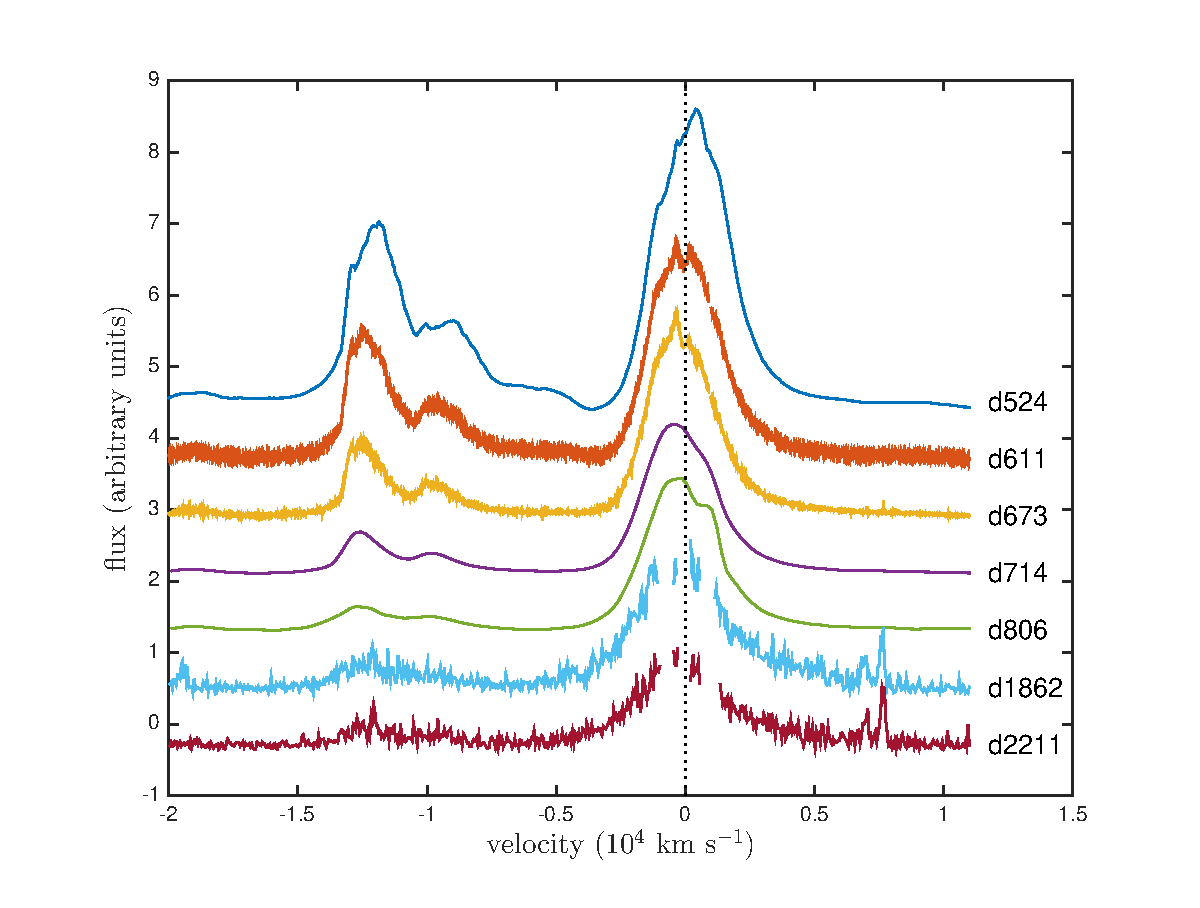
\includegraphics[trim =39 10 45 15,clip=true,scale=0.51]{Ha_evol_early_1col}
\caption{Archival data showing the evolution of the H$\alpha$ and
[O~{\sc i}] line profiles from SN~1987A at the earlier epochs. The 
spectral gaps at the last two epochs correspond to where narrow line 
emission from the equatorial ring has been removed. The spectra have been
continuum-subtracted and offsets applied for display purposes.}
\label{Ha_evol_early}
%\end{center}
\end{figure}
%!!!!!!!!!!!!FIG!!!!!!!!!!!!!!!!!!

%%%%%%%%%%%%%%%%%%%%   SPECTRA   %%%%%%%%%%%%%%%%%%%%%%%%%%%

\section{Archival spectra of SN 1987A}
\label{spectra}

SN~1987A has been the most intensively observed supernova in history, with 
a wealth of both spectral and photometric data available to model.  From 
the archives of a number of different telescopes we have collated optical 
spectra acquired over a wide range of epochs.  At the earlier epochs we 
use spectra obtained with the Anglo-Australian Telescope (AAT) and Cerro 
Tololo Inter-American Observatory (CTIO) and at later epochs we 
use spectra from the archives of the Hubble Space Telescope (HST) and Very 
Large Telescope (VLT).  An explosion date of 23 February 1987 is adopted 
throughout and epochs are measured relative to this date.  Full details of 
all observations may be found in Table \ref{tb:data}. The spectral 
resolutions of the grating spectrograph observations are listed in 
column~7, while column 8 lists the spectral resolving powers of the 
echelle spectrograph observations.

Wavelength ranges encompassing the H$\alpha\ $ line and [O~{\sc i}] 
$\lambda$6300,6363~\AA\ doublet were selected in order to trace their 
evolution from day 524, near the time of the first indications of dust 
formation (Wooden et al. 1993) to day 8020, near the current era. Optical 
spectroscopy obtained at the AAT using the Faint Object Red Spectrogaph 
(FORS) during the first two years was kindly supplied by Dr Raylee 
Stathakis \citep{Spyromilio1991, Spyromilio1993a, Hanuschik1993}.

The evolution of the H$\alpha$ line profile is presented in Figures 
\ref{Ha_evol_early} and \ref{Ha_evol_late}.  At later epochs, the broad 
profile emitted by the ejecta becomes contaminated by narrow line emission 
from the equatorial ring.  These lines have been removed for the purposes 
of modelling the broad line. A continuum fit has been subtracted from each 
spectrum and a velocity correction has been applied for a recession 
velocity of 287 km~s$^{-1}$ \citep{Groningsson2008}.

\begin{table*}
	\begin{minipage}{180mm}
	\caption{Details of the archival data for SN 1987A}
	\label{tb:data}
  	\begin{tabular}{@{} ccccccccl @{}}
    	\hline
	Date & Age & Telescope  & Inst & $\lambda_{min}$ & $\lambda_{max}$ & Res. & Res. Power & Reference \\
	& (days) & & &(\AA) & (\AA)& (\AA)\\
	\hline
31 Jul 1988 & 524 & AAT & FORS & 5500 & 10190 & 20 & & \citet{Spyromilio1991} \\
26 Oct 1988 & 611 & AAT & UCLES & 6011 & 7336 &  & 30000 & \citet{Hanuschik1993, Spyromilio1993a}\\
27 Dec 1988 & 673 & AAT & UCLES & 5702 & 10190 &  & 30000 & \citet{Hanuschik1993, Spyromilio1993a}\\
06 Feb 1989 & 714 & CTIO-1.5m & Cass. & 6420 & 10380 & 16 & & \citet{Phillips1990}\\
09 May 1989 & 806 & CTIO-1.5m & Cass. & 6430 & 10330 & 16 & & \citet{Phillips1990}\\
30 Mar 1992 & 1862 & HST & STIS & 4569 & 6818 & 4.4 &  & \citet{Wang1996}\\
14 Mar 1993 & 2211 & HST & STIS & 4569 & 6818 & 4.4 &  & \citet{Wang1996}\\
07 Jan 1995 & 2875 & HST & STIS & 4569 & 6818 & 4.4 &  & \citet{Chugai1997}\\
23 Sep 1996 & 3500 & HST & STIS & 4569 & 6818 & 4.4 &  \\
05 Jan 1997 & 3604 & HST & STIS & 4569 & 6818 & 4.4 &  \\
10 Dec 2000 & 5039 & VLT & UVES & 4760 & 6840 &  & 50000 & \citet{Groeningsson2006, Groeningsson2007}\\
06 Oct 2002 & 5704 & VLT & UVES & 4760 & 6840 &  & 50000 & \citet{Groeningsson2006, Groeningsson2007, Groningsson2008}\\
21 Mar 2005 & 6601 & VLT & UVES & 4760 & 6840 &  & 50000 &\citet{Groeningsson2006, Groeningsson2007}\\
23 Oct 2007 & 7547 & VLT & UVES & 4760 & 6840 &  & 50000 & \citet{Groeningsson2007}\\
07 Feb 2009 & 8020 & VLT & UVES & 4800 & 6800 &  & 50000 & \citet{Tziamtzis2010}\\
    \hline
  \end{tabular}
\end{minipage}
\end{table*}



\begin{figure}
%\begin{center}
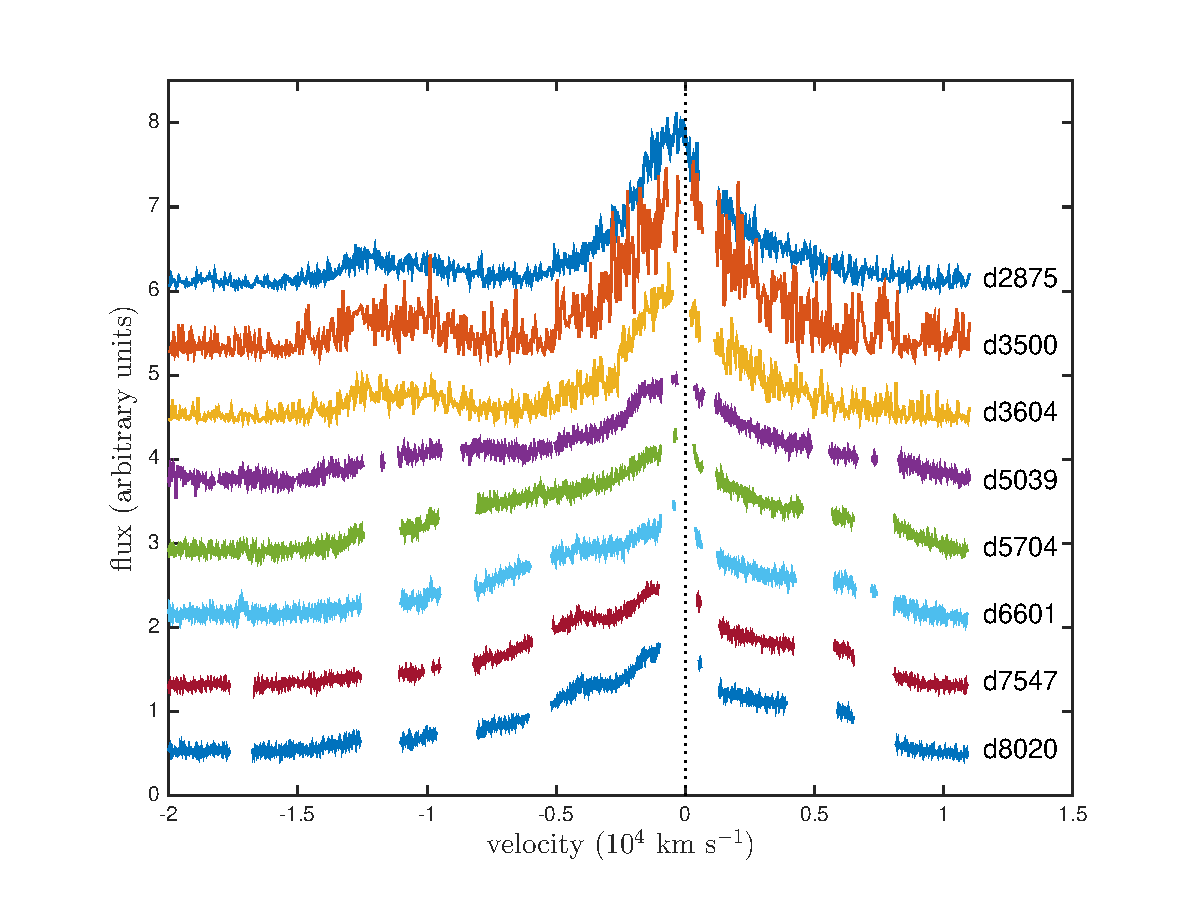
\includegraphics[trim =45 10 45 15,clip=true,scale=0.51]{Ha_evol_late_1col}
\caption{Archival data showing the evolution of the H$\alpha$
line profile from SN~1987A at the later epochs. The spectral gaps 
correspond to where narrow line emission from the equatorial ring has been 
removed. The spectra have been continuum-subtracted and offsets applied 
for display purposes.}
\label{Ha_evol_late}
%\end{center}
\end{figure}

%%%%%%%%%%%%%%%%%%%%   SPECTRA   %%%%%%%%%%%%%%%%%%%%%%%%%%%
%%%%%%%%%%%%%%%%%%%%   CODE   %%%%%%%%%%%%%%%%%%%%%%%%%%%
\section{The DAMOCLES code}
\label{code}

Monte Carlo methods have long been used to model radiative transfer 
problems in diverse environments and there are several examples of codes 
which utilise the technique in application to supernovae 
\textit{(references)}.  Whilst there are numerous codes that 
treat dust or gas or both in order to produce an overall spectral energy 
distribution (SED), there is a dearth of codes designed to focus on the 
shapes of single line profiles.  Although a velocity field is naturally 
considered in codes that seek to reproduce the spectra of supernovae, 
absorption and scattering by dust is not and thus the resulting shapes of 
line profiles are potentially unrepresentative of those emerging from 
dusty ejecta.

In this work we aim to model single line profiles or doublets produced by 
a moving atmosphere in a dusty medium.  
Since a comparatively small wavelength range is considered, a fully 
self-consistent radiative transfer model is unnecessarily expensive.  
Instead any energy packet that is absorbed during the simulation may 
simply be removed from circulation on the grounds that it would be 
reemitted outside the wavelength range of interest. The extinction due to 
dust is assumed to be temperature-independent and it is therefore 
unnecessary to iteratively calculate the temperature of the ejecta as in a 
fully self-consistent calculation of the SED.  Though clearly the total 
energy transferred through the medium is not conserved, the signature of 
the normalised line profile is preserved.

The DAMOCLES code builds on the work of \citet{Lucy1989a} who employed a 
similar approach to model the broad [O~{\sc i}] $\lambda 6300~\AA\ line 
seen in SN~1987A at early epochs ($\sim$ day 775).  It models the 
transport of initially monochromatic energy packets through a smooth or 
clumped dusty medium having a smooth velocity field. The velocity field 
and the inner an outer ejecta radii are free parameters. The late-time 
($>$400 days) line emission is assumed to be optically thin, with an 
emissivity proportional to the square of the local gas density, e.g. 
propertional to the product of the recombining proton and electron 
densities in the case of H$\alpha$ and to the product of the neutral 
oxygen and electron densities in the case of collisionally excited [O~{\sc 
i}] emission.

\subsection{The energy packets formalism}
\label{packets}

The initial radiation field is inherently tied to the distribution of gas 
throughout the supernova ejecta which is declared as a power law $\rho(r) 
\propto r^{-\beta}$ between $R_{in}$ and $R_{out}$. The emissivity 
distribution is also specified as a power law with $i(\rho) \propto 
\rho^{k}$.  However this is generally taken to be $i(r) \propto r 
^{-2\beta}$ since the majority of lines modelled are recombination lines 
and therefore $i(\rho) \propto \rho^2$.  The radiation is quantised into 
monochromatic packets with equal energy $E_{0}=nh\nu_{0}$.  In Monte Carlo 
simulations that model non-moving atmospheres, packets are usually taken 
to be of constant energy.  When the frequency of a packet is altered after 
an event, the energy of that packet is kept constant and the number of 
real photons contained within it assumed to change.  However, in the case 
of dust scattering, the number of real photons is conserved and thus the 
energy of the packet is altered.  This is most easily achieved by 
weighting each packet over all scattering events as \[w=\prod_{scat} 
\frac{\nu'}{\nu}\] where $w$ is the weight of the packet.  The final 
energy of each packet is then $E=wE_0$, where $E_0$ is the initial energy 
of the packet.

The supernova ejecta is divided into shells between $R_{in}$ and $R_{out}$ 
and the number of packets to be emitted in each shell calculated according 
to the emissivity distribution and emitted isotropically.  For each packet 
a location within that shell and an initial trajectory is randomly sampled 
from an isotropic distribution such that

\begin{equation}
\phi=2\pi\eta
 \cos \theta=2\xi -1
\end{equation}

\noindent where $0<\eta<1$ and $0<\xi<1$ are random numbers, $\phi$ is the 
azimuthal angle and $\cos \theta$ is the radial direction cosine.  At 
emission and at each scattering event the frequency of the packet is 
recalculated according to the specified radial velocity field $v(r) 
\propto v_{max}r^{\alpha}$ (see section \ref{transport}) .


\begin{figure*}
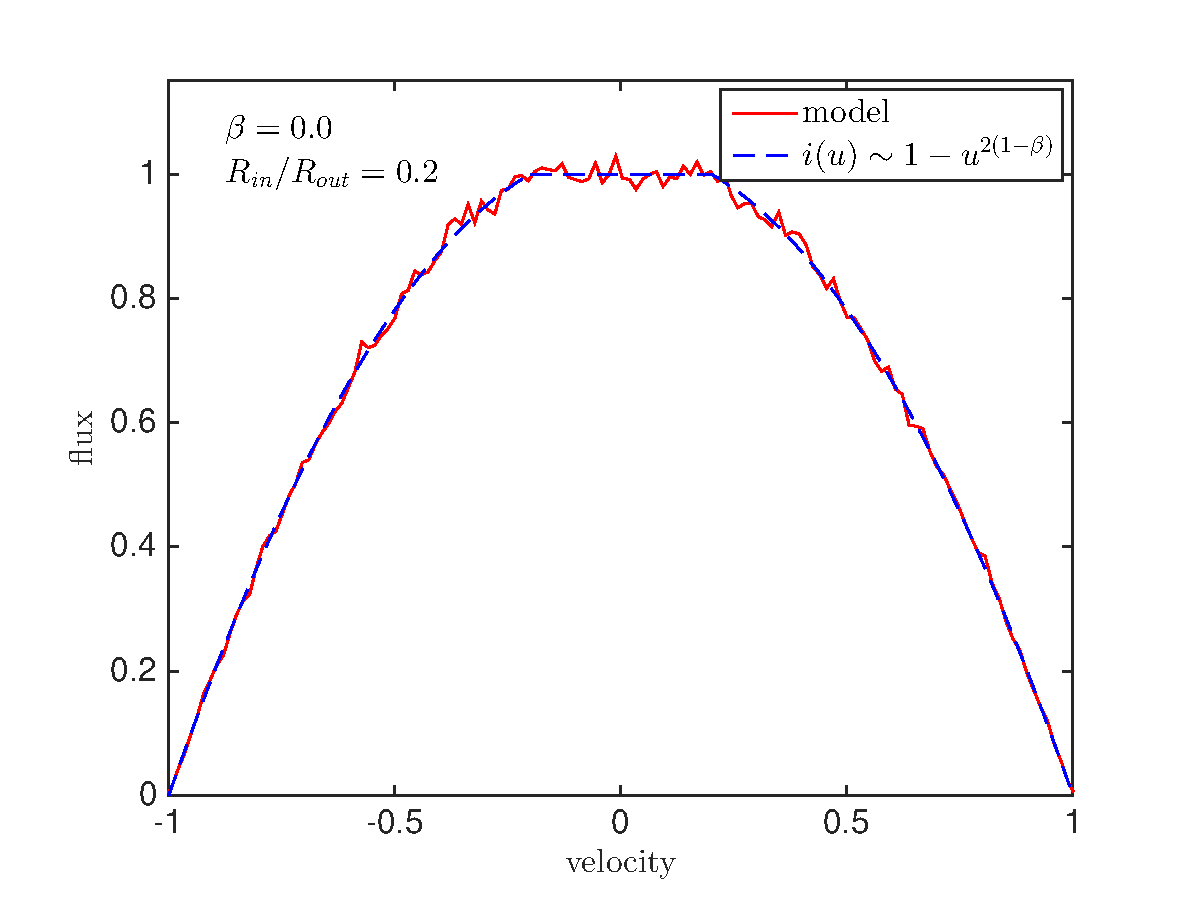
\includegraphics[trim =25 25 45 15,clip=true,scale=0.34]{params/A/b0_r0_2} 
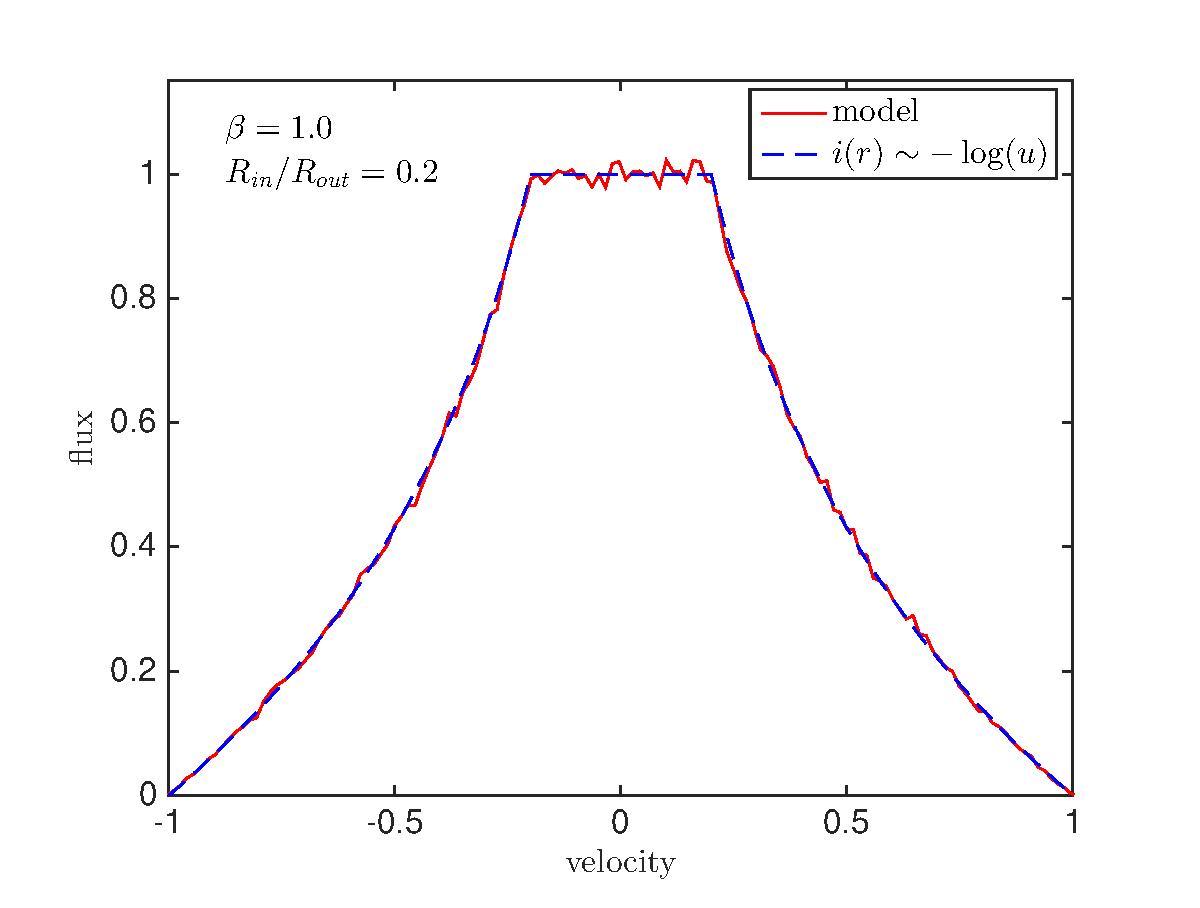
\includegraphics[trim =37 25 45 15,clip=true,scale=0.34]{params/A/b1_r0_2}
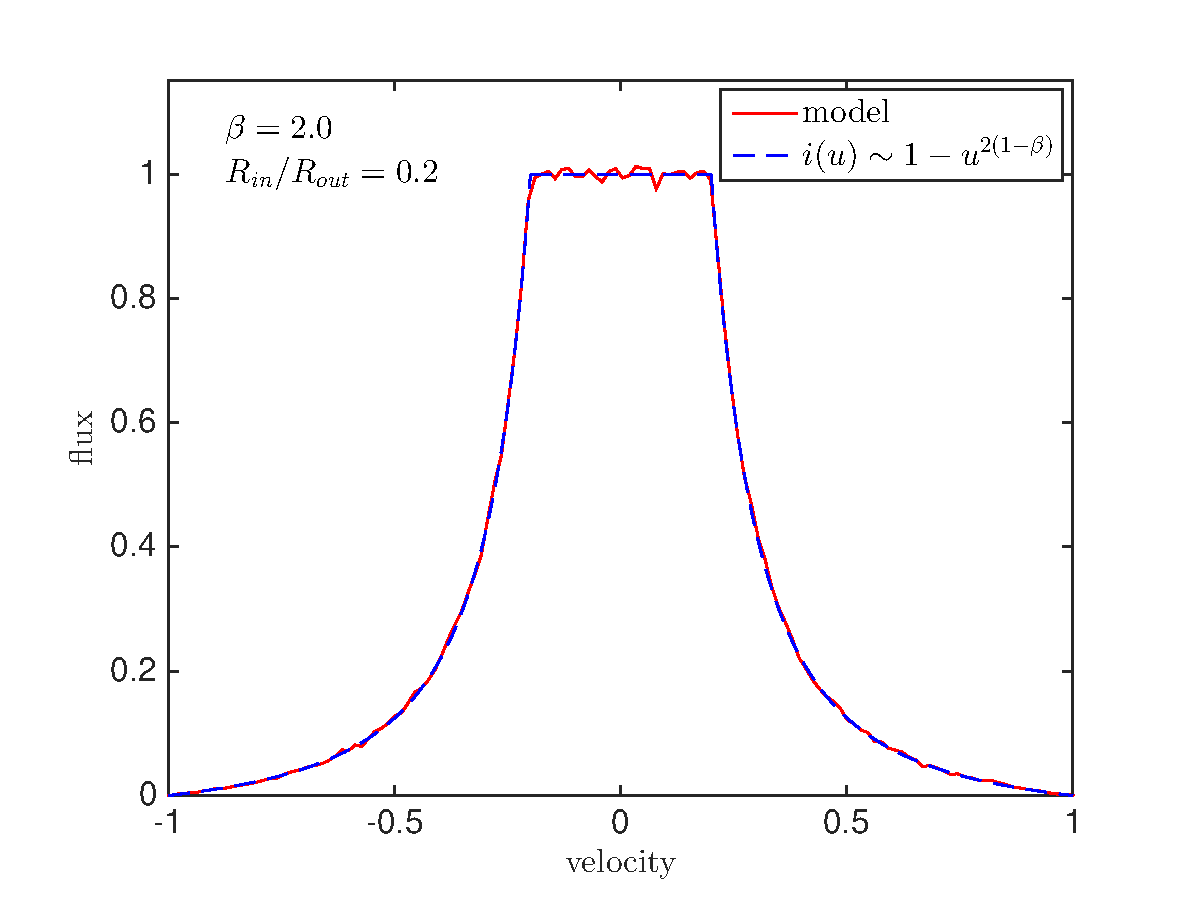
\includegraphics[trim =37 25 45 15,clip=true,scale=0.34]{params/A/b2_r0_2}
\\
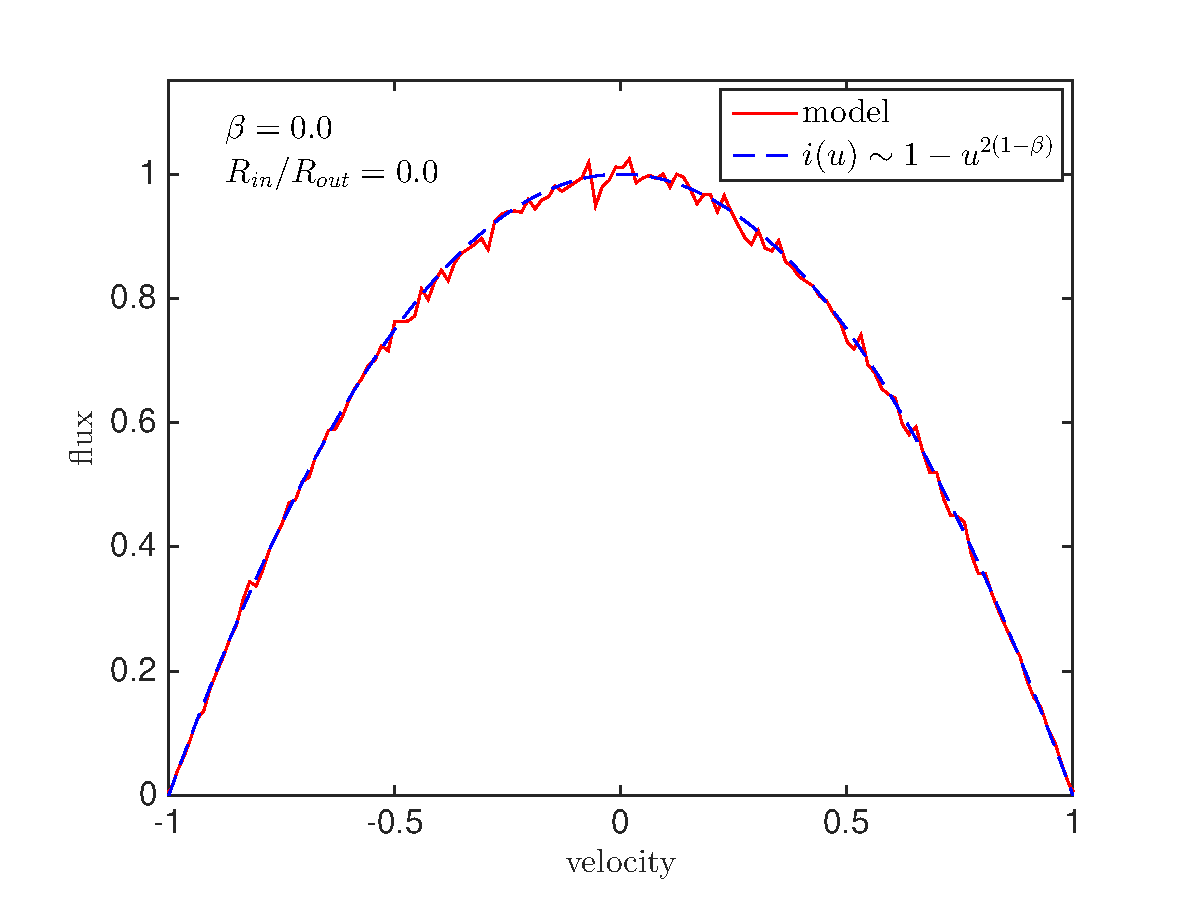
\includegraphics[trim =25 5 45 15,clip=true,scale=0.34]{params/A/b0_r0}  
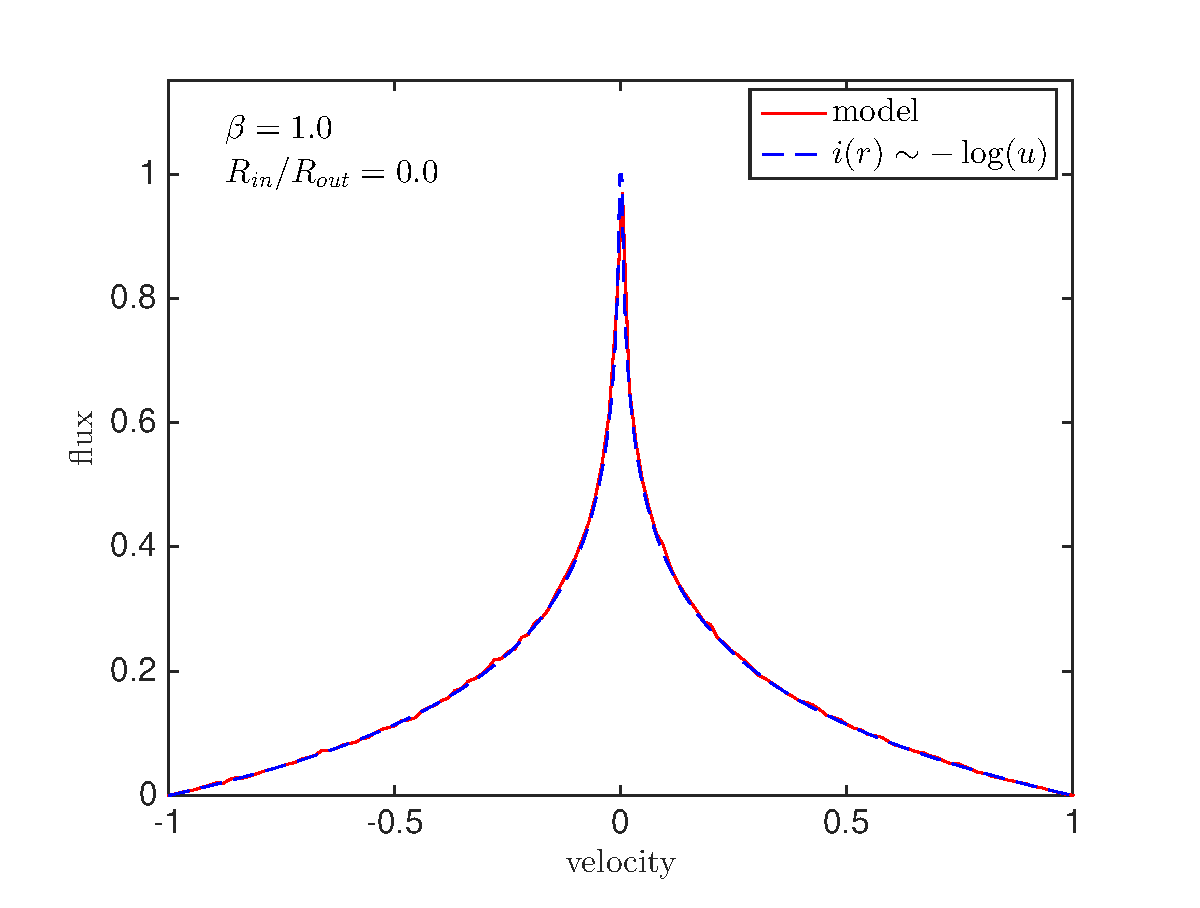
\includegraphics[trim =37 5 45 15,clip=true,scale=0.34]{params/A/b1_r0} 
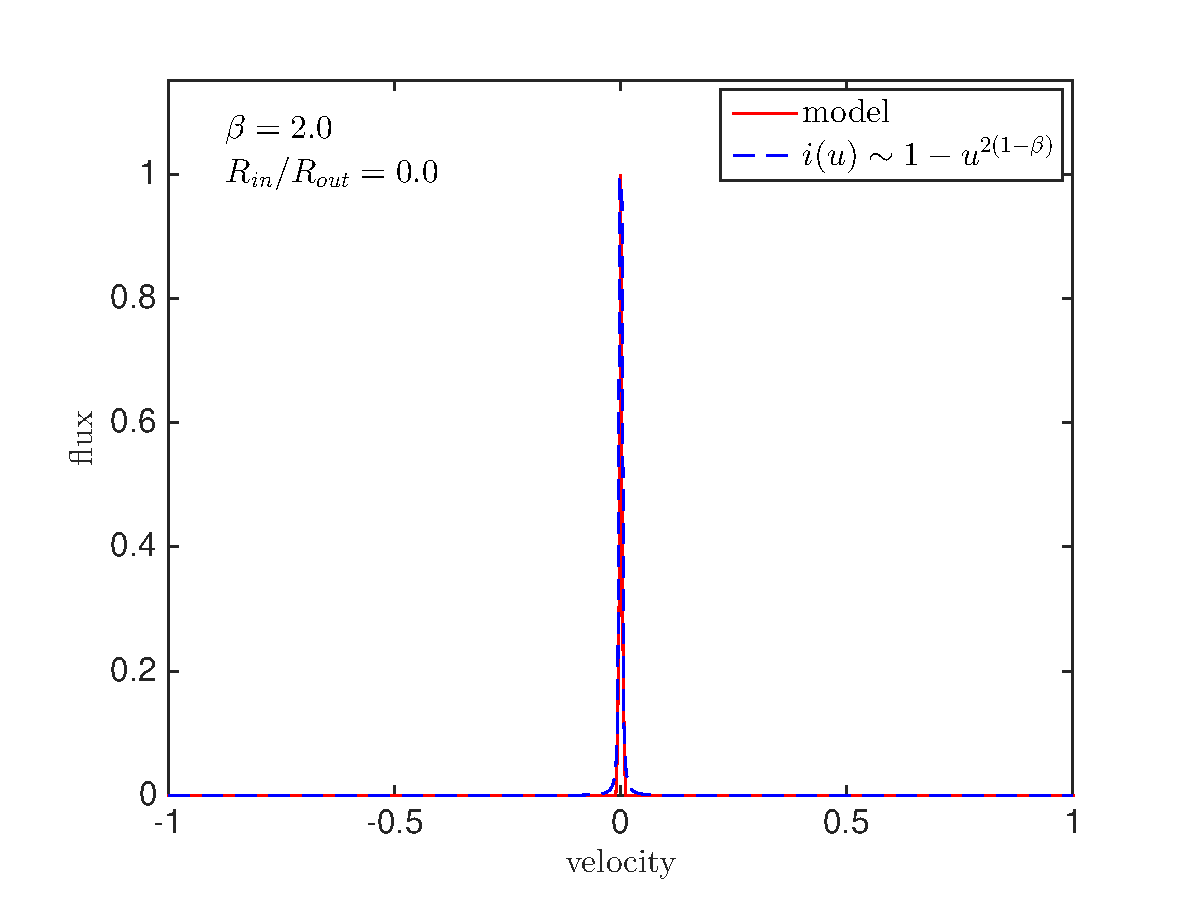
\includegraphics[trim =37 5 45 15,clip=true,scale=0.34]{params/A/b2_r0}

\caption{\textit{Red:} Benchmark models of optically thin ($\tau =0$) 
line profiles  with $v \propto r$. Left to right: initial emissivity 
profiles are $i(r) \propto r^{-2\beta}$ with $\beta=0.0$, $\beta=1.0$ and 
$\beta=2.0$. Cases with $R_{in}/R_{out}=0.2$ are on the top and 
$R_{in}/R_{out}=0.0$ on the bottom.  \textit{Blue:} The analytical case 
with $i(u) \sim 1-u^{2(1-\beta)}$ except in the case of $\beta=1$ where 
$i(u) \sim -\log u$.}
\label{fig:analytics}
\end{figure*}

\subsection{The geometry of the ejecta and the grid}
\label{grid}

The supernova ejecta is approximated by a three-dimensional cartesian 
grid, each cell of which is assumed to have uniform density and 
composition.  The grid is a cube with sides of width $2R_{out}$ and a 
declarable number of divisions.  After the initial emission of energy 
packets, the gas plays no further role in the simulation and thus only 
dust properties are considered.  By default, the dust is coupled to the 
gas (although it may be decoupled) and thus follows the smooth 
distribution described above ($\rho \propto r^{-\beta}$).  The dust 
density in each cell is therefore calculated accordingly and any cell 
whose centre falls outside of the bounds of the supernova ejecta has 
density set to zero.

It is worth noting that if a constant mass loss rate is required, the 
exponent of the velocity profile and the exponent of the density profile 
are not independent.  A constant mass loss rate implies that $4\pi \rho 
vR^2 \propto k$, where $k$ is a constant, and thus for $v \propto 
r^\alpha$ and $\rho\propto r^{-\beta}$, we require that $\beta-\alpha=2$.  
However, it is possible that the supernova event may have induced a 
mass-flow rate that is not constant with radius and thus both exponents 
may be declared independently.

It is known from SED modelling that clumped environments produce very 
different results to environments assumed to have a smooth distribution of 
dust and gas.  Specifically, clumped models tend to require more dust in 
order to reproduce a similar level to a smoothly distributed model.  The 
capacity for modelling a clumped dusty medium is therefore included in the 
code.  The fraction of the dust mass that is in clumps is declared 
($m_{frac}$) and the total volume filling factor of the clumps ($f$) is 
also specified.  Dust that is not located in clumps is distributed 
according to a smooth radial profile.  The clumps occupy a single grid 
cell and their size can therefore be varied by altering the number of 
divisions in the grid.  They are distributed stochastically with 
probability of a given cell being a clump proportional to the smooth 
density profile (i.e. $p(r) \propto r^{-\beta}$).  The density of all 
clumps is constant and is calculated as

\begin{equation}
\rho_{clump}=\frac{M_{clumps}}{V_{clumps}}=\frac{m_{frac}M_{tot}}{\frac{4}{3} f\pi (R_{out}^{3}-R_{in}^{3} )}
\end{equation}

\noindent where $M_{tot}$ is the total dust mass, $M_{clumps}$ is the 
total dust mass in clumps and $V_{clumps}$ is the total volume occupied by 
clumps.  $m_{frac}$ and $f$ are defined as above.


\subsection{The radiative transport mechanism}
\label{transport}

Following emission a packet must be propagated through the grid until it 
escapes the outer bound of the ejecta $R_{out}$.  The probability that the 
packet travels a distance $l$ without interacting is $p(l)=e ^{-n \sigma 
l}=e ^{-\tau} $ where $n$ is the number density, $\sigma$ is the 
cross-section of interaction and $ \tau = n\sigma l$ for constant $n$ and 
$\sigma$ (as in a grid cell).  Noting that the probability that a packet 
does interact within a distance $l$ is therefore $1-e^{-\tau}$, we may 
sample from the cumulative probability distribution to give:

\begin{equation}
\xi = 1 - e^{-\tau}   \tau=-\log (1-\xi)
\end{equation}

\noindent where $0<\xi<1$ is a sampled random number set to be the value 
of the optical depth for that packet in that cell.  The frequency of the 
photon packet and the mass density of the cell are then used to calculate 
the opacity of that cell and, using the fact that $n\sigma=\kappa\rho$, 
the distance $l$ that the packet travels before its next interaction is 
calculated.  If this value is greater than the distance from its position 
to the edge of the cell then the packet is moved along its current 
trajectory to the cell boundary and the process is repeated.  If the 
distance is less than the distance to the boundary then an event occurs 
and the packet is either scattered or absorbed with probability of 
scattering equal to the albedo of the cell

\begin{equation}
	\omega=\frac{\sigma_{sca}}{\sigma_{sca}+\sigma_{abs}}
\end{equation}

If the packet is absorbed then it is simply removed from the simulation as 
discussed above.  If the packet is scattered then a new trajectory is 
sampled from an isotropic distribution in the comoving frame of the dust 
grain and the frequency of the packet recalculated using Lorentz 
transforms subject to the velocity at the radius of the interaction (see 
appendix A for further details).  This process is repeated until the 
packet has either escaped the outer bound of the supernova ejecta or been 
absorbed.
   
Escaped packets are added to frequency bins weighted by $w$ in order to 
produce an overall emergent line profile.


\subsection{Properties of the Dusty Medium}

Dust of any composition may be used for which optical data is available 
and the relative abundances of the species may be declared by the user.  
A grain size may be specified for each species.  Since a full radiative 
transfer calculation is not performed, it is not useful to specify a grain 
size distribution since the extinction to dust is only dependent on the 
cross-sectional area of the grains and not to the overall distribution.  
The capacity to declare a size distribution is however included for the 
sake of ease of comparison with SED models.  A Mie approximation is used 
to calculate the overall $Q_{abs}(\nu)$ and $Q_{sca}(\nu)$ for each 
species and the derived opacities are summed over each species weighted 
according to their relative abundances.


As will be discussed in sections \ref{params}, the effects of scattering 
on the shapes of line profiles can potentially be quite pronounced and it 
is therefore important to consider the potential effects of electron 
scattering as well as those of dust scattering.  Electron densities are 
calculated using an estimated average temperature and observed luminosity 
of $H_{\alpha}$ and the optical depth to electrons calculated from this.  
Electron scattering is treated in an identical manner to dust scattering 
with with $\tau = \tau_{dust}+\tau_{e}$ in each cell.  If, for a given 
packet, an event ocurrs, it is first calculated whether this is a dust 
event or a scattering event by considering the ratio of the optical depths 
to each species.  If the packet is scattered by an electron then this 
process is identical to dust.  If not, then the process continues as 
described above.

In the majority of cases it seems that the electron densities are not high 
enough to discernibly effect the overall shape of the profile.  However, 
there may be a few rare cases (the concept is discussed for SN 2010jl 
\citep{Fransson2013}) where the electron densities are high enough to 
become significant in the observed profiles.  Whilst the inclusion of 
electron scattering in the code is an approximation, it gives a good 
suggestion of the potential effects of electron scattering.

%%%%%%%%%%%%%%%%%%%%   CODE   %%%%%%%%%%%%%%%%%%%%%%%%%%%


%%%%%%%%%%%%%%%%%%%%   TESTING/PARAMS   %%%%%%%%%%%%%%%%%%%%%%%%%%%
\section{Comparison of DAMOCLES models with analytical and previously published results}
\label{params}

There is a general lack of published models in the literature that 
consider absorption-affected asymmetric line profiles.  We therefore test 
the code by comparing the results to optically thin profiles that may be 
derived analytically.  We then test the absorption and scattering 
components of the code by comparing our results in the case of an 
optically thick medium with those derived by \citet{Lucy1989a} in their 
Model II and Model III scenario.

\subsection{Comparison of DAMOCLES models with analytical results}
\label{analytics}

Analytical profiles may be calculated in the dust-free case.  I run a 
number of models based on mathematics derived by \cite{Gerasimovic1933} 
that derive the equations of line profiles emitted from a transparent 
expanding shell in the field of a star.

Describing the expansion velocity of the shell as $v=r^\alpha$ with 
$\alpha \neq 0$ and maximum velocity $v_{max}=1$, the energy emitted by 
the nebula between radial velocities $v$ and $v+dv$ is proportional to

\begin{equation}
\int _\tau i(r) r \sin (\theta) r d\theta dr
\end{equation}

\noindent where $i(r)$ represents the emission per unit volume at radius 
$r$.  We adopt inner radius $R=q$ and outer radius $R=1$.

Setting $i(r) \propto r^{-2\beta}$ (for a recombination line emitted from 
a medium with assumed density profile for the emitter $\rho \propto 
r^{-\beta}$) then gives

\begin{equation}
\begin{split}
i(v)dv &\sim \frac{dv}{\alpha v^{\frac{2\beta-3+\alpha}{\alpha}}} \int^{\theta_1}_{\theta_0} \cos^{\frac{2\beta-3}{\alpha}} \theta \sin \theta d\theta 
\\
&\sim  \frac{dv}{v^{\frac{2\beta-3+\alpha}{\alpha}}} \Bigg[\frac{\cos^{\frac{2\beta - 3 + \alpha}{\alpha}} \theta}{2\beta -3 + \alpha}\Bigg]^{\theta_0}_{\theta_1}
\end{split}
\end{equation}

\noindent for $\frac{2\beta-3}{\alpha} \neq -1$.  The case 
$\frac{2\beta-3}{\alpha} = -1$ results in a logarithmic relationship.


In the case of a "complete" nebula, i.e. one where the inner radius is 
vanishingly small in comparison to the outer radius, we obtain

\begin{equation}
\label{eqn:sides}
	i(v) dv \sim \pm \frac{du}{(2\beta-3+\alpha) v^{\frac{2\beta-1+\alpha}{\alpha}}} \Big(1-v^{\frac{2\beta-3+\alpha}{\alpha}} \Big)
\end{equation}

If the nebula is not "complete", that is to say, the inner radius is of the order of the outer radius and the remnant is a detached shell, the above formula becomes valid only from $v=1$ to some critical value $v'=q^\alpha$. For $v<v'$, we obtain

\begin{equation}
i(v)dv \sim \pm \frac{dv}{(2\beta-3+\alpha)} \Big( \frac{1}{q^\alpha} - 1 \Big)
\end{equation}

\noindent and therefore the top of the line is flat while the sides are 
sloping.

Crucially, the width of the flat section is determined by $v'=q^\alpha$ or 
simply $v'=q$ in the case where $v \propto r$, whilst the shape of the 
profile outside of the flattop is described by equation \ref{eqn:sides}.

Profiles of a variety of shapes may be derived from these formulae 
depending on the relative values of $\alpha$ and $\beta$.  Here we 
consider three main families of curves:


%\begin{minipage}{0.55\textwidth}
\begin{enumerate}\parskip3pt

	\item \ \ $\quad i(v)  \sim v^{-\gamma}-1$ \quad ($\alpha>0$, $2\beta-3+\alpha>0$)
	\item \ $\quad i(v)  \sim 1-v^\gamma$ \quad \ \ ($\alpha>0$, $2\beta-3+\alpha<0$)
	\item  $\quad i(v) \sim -\log v$ \quad \ \ ($\alpha>0$, $2\beta-3+\alpha=0$)

\end{enumerate}
%\end{minipage}


\noindent where $\gamma$ is defined as $\gamma= \lvert 
\frac{2\beta-3+\alpha}{\alpha} \rvert$.

Models are presented for each of these cases, both in the environment of a 
complete nebula and one with a shell structure with $R_{in}/R_{out}=0.2$.  
A velocity profile $v \propto r$ appropriate for a supernova in the free 
expansion phase is used throughout.  Values of $\beta = 0, 1$ and $2$ are 
adopted.  Figure \ref{fig:analytics} illustrates the perfect fit between 
the analytical case and the model.  Fluxes are scaled to 1 at the peak.

\subsection{Comparison of DAMOCLES models with previously published results}
\label{opt_thick_testing}
\begin{figure*}
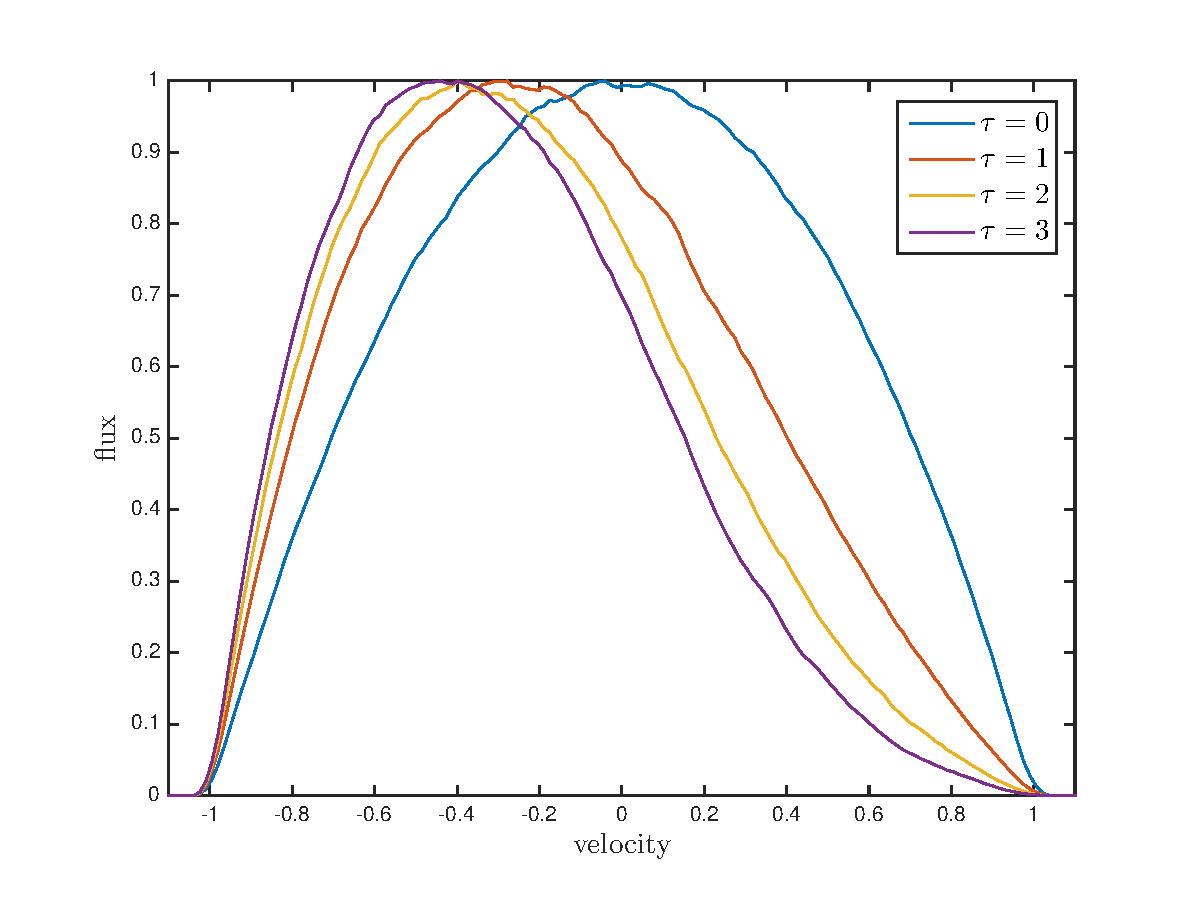
\includegraphics[trim =37 10 45 15,clip=true,scale=0.51]{params/opt_thick_w0} 
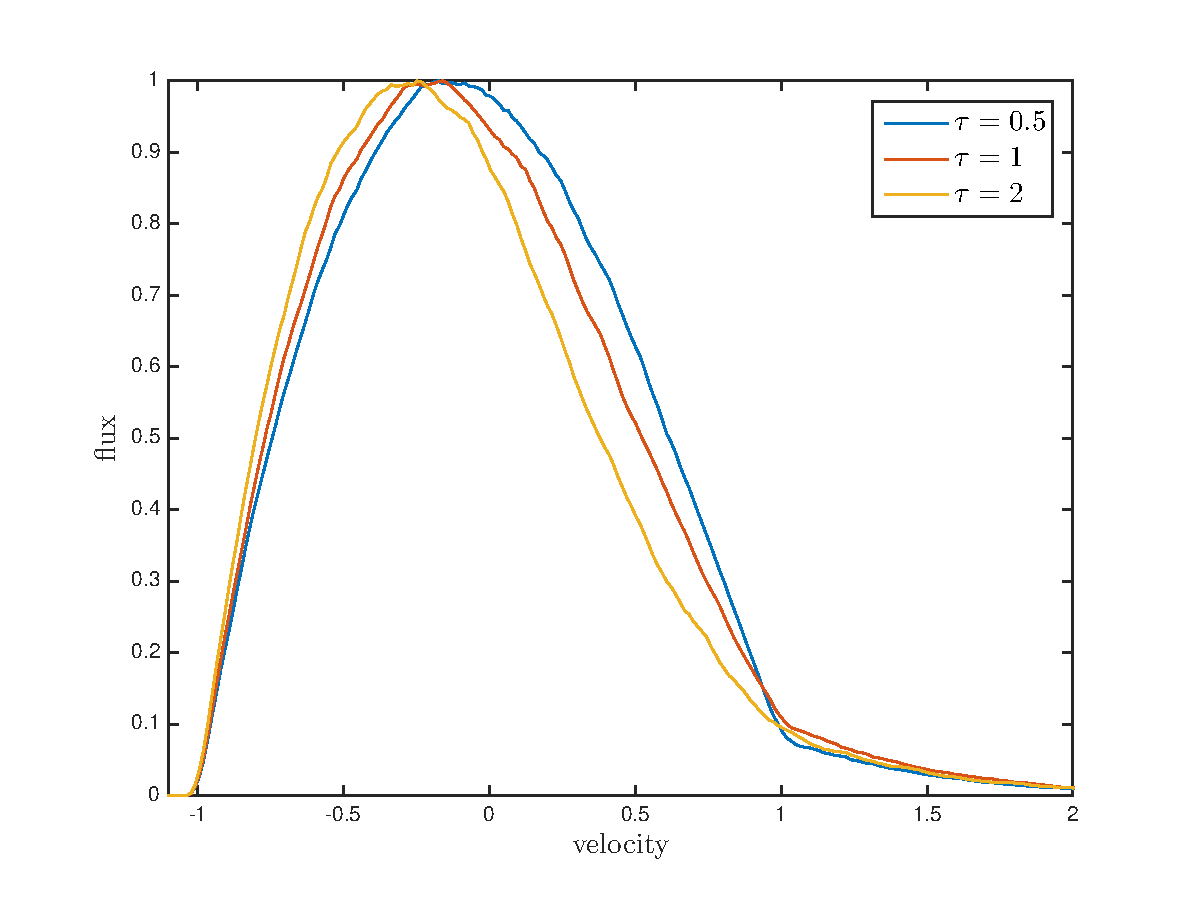
\includegraphics[trim =37 10 45 15,clip=true,scale=0.51]{params/opt_thick_w0_6}  
\caption{Benchmark models of optically thick line profiles  with $v \propto r$, $i(r) \propto$ constant and $R_{in}/R_{out}=0$.  Pure absorption models ($\omega = 0$) are presented on the left, partially scattering models are presented on the right ($\omega = 0.6$) as per \citet{Lucy1989a} Models II and III.}
\label{fig:Lucy}
\end{figure*}


In addition to the optically thin testing described above, we also 
compared our outputs to those derived by \citet{Lucy1989a} in order to 
assess the accuracy of the scattering and absorption aspects of the code.  
We consider two similar cases equivalent to Models II and III in the 
\citet{Lucy1989a} paper. In the first case, dust with zero albedo is 
uniformly distributed throughout a complete nebula with velocity profile 
$v \propto r$.  In the second, the same scenario is considered but a 
medium of dust with $\omega =0.6$ is considered.

In the first case, the profile may once again be derived analytically from 
the basic geometry using the fact that radiation will be attenuated by a 
factor $e^{-2\tau v}$ between points with line of sight velocity $-v$ and 
$v$.  The line profile is therefore given by

\[
I(v) = I(-v)\exp(-2\tau v)  
\]

\citet{Lucy1989a} present several examples of both the analytical case of 
the perfect absorber and a Monte Carlo model for a grain with $\omega 
=0.6$.  We present the same cases in figure \ref{fig:Lucy} and note that 
the resulting profiles exhibit the same features and shape. Of particular 
interest is the scattering wing that appears beyond the maximum velocity 
($v_{max}=1$) on the red side of profiles in the case of the partial 
scatterer as a result of the packets doing work on the expanding sphere.  
This is noted by \citet{Lucy1989a} as a potential diagnostic for the 
presence of dust in the ejecta of a supernova and we will discuss this 
further in section \ref{ps}.


\subsection{The sensitivity of the variable parameters}
\label{ps}

\begin{figure*}
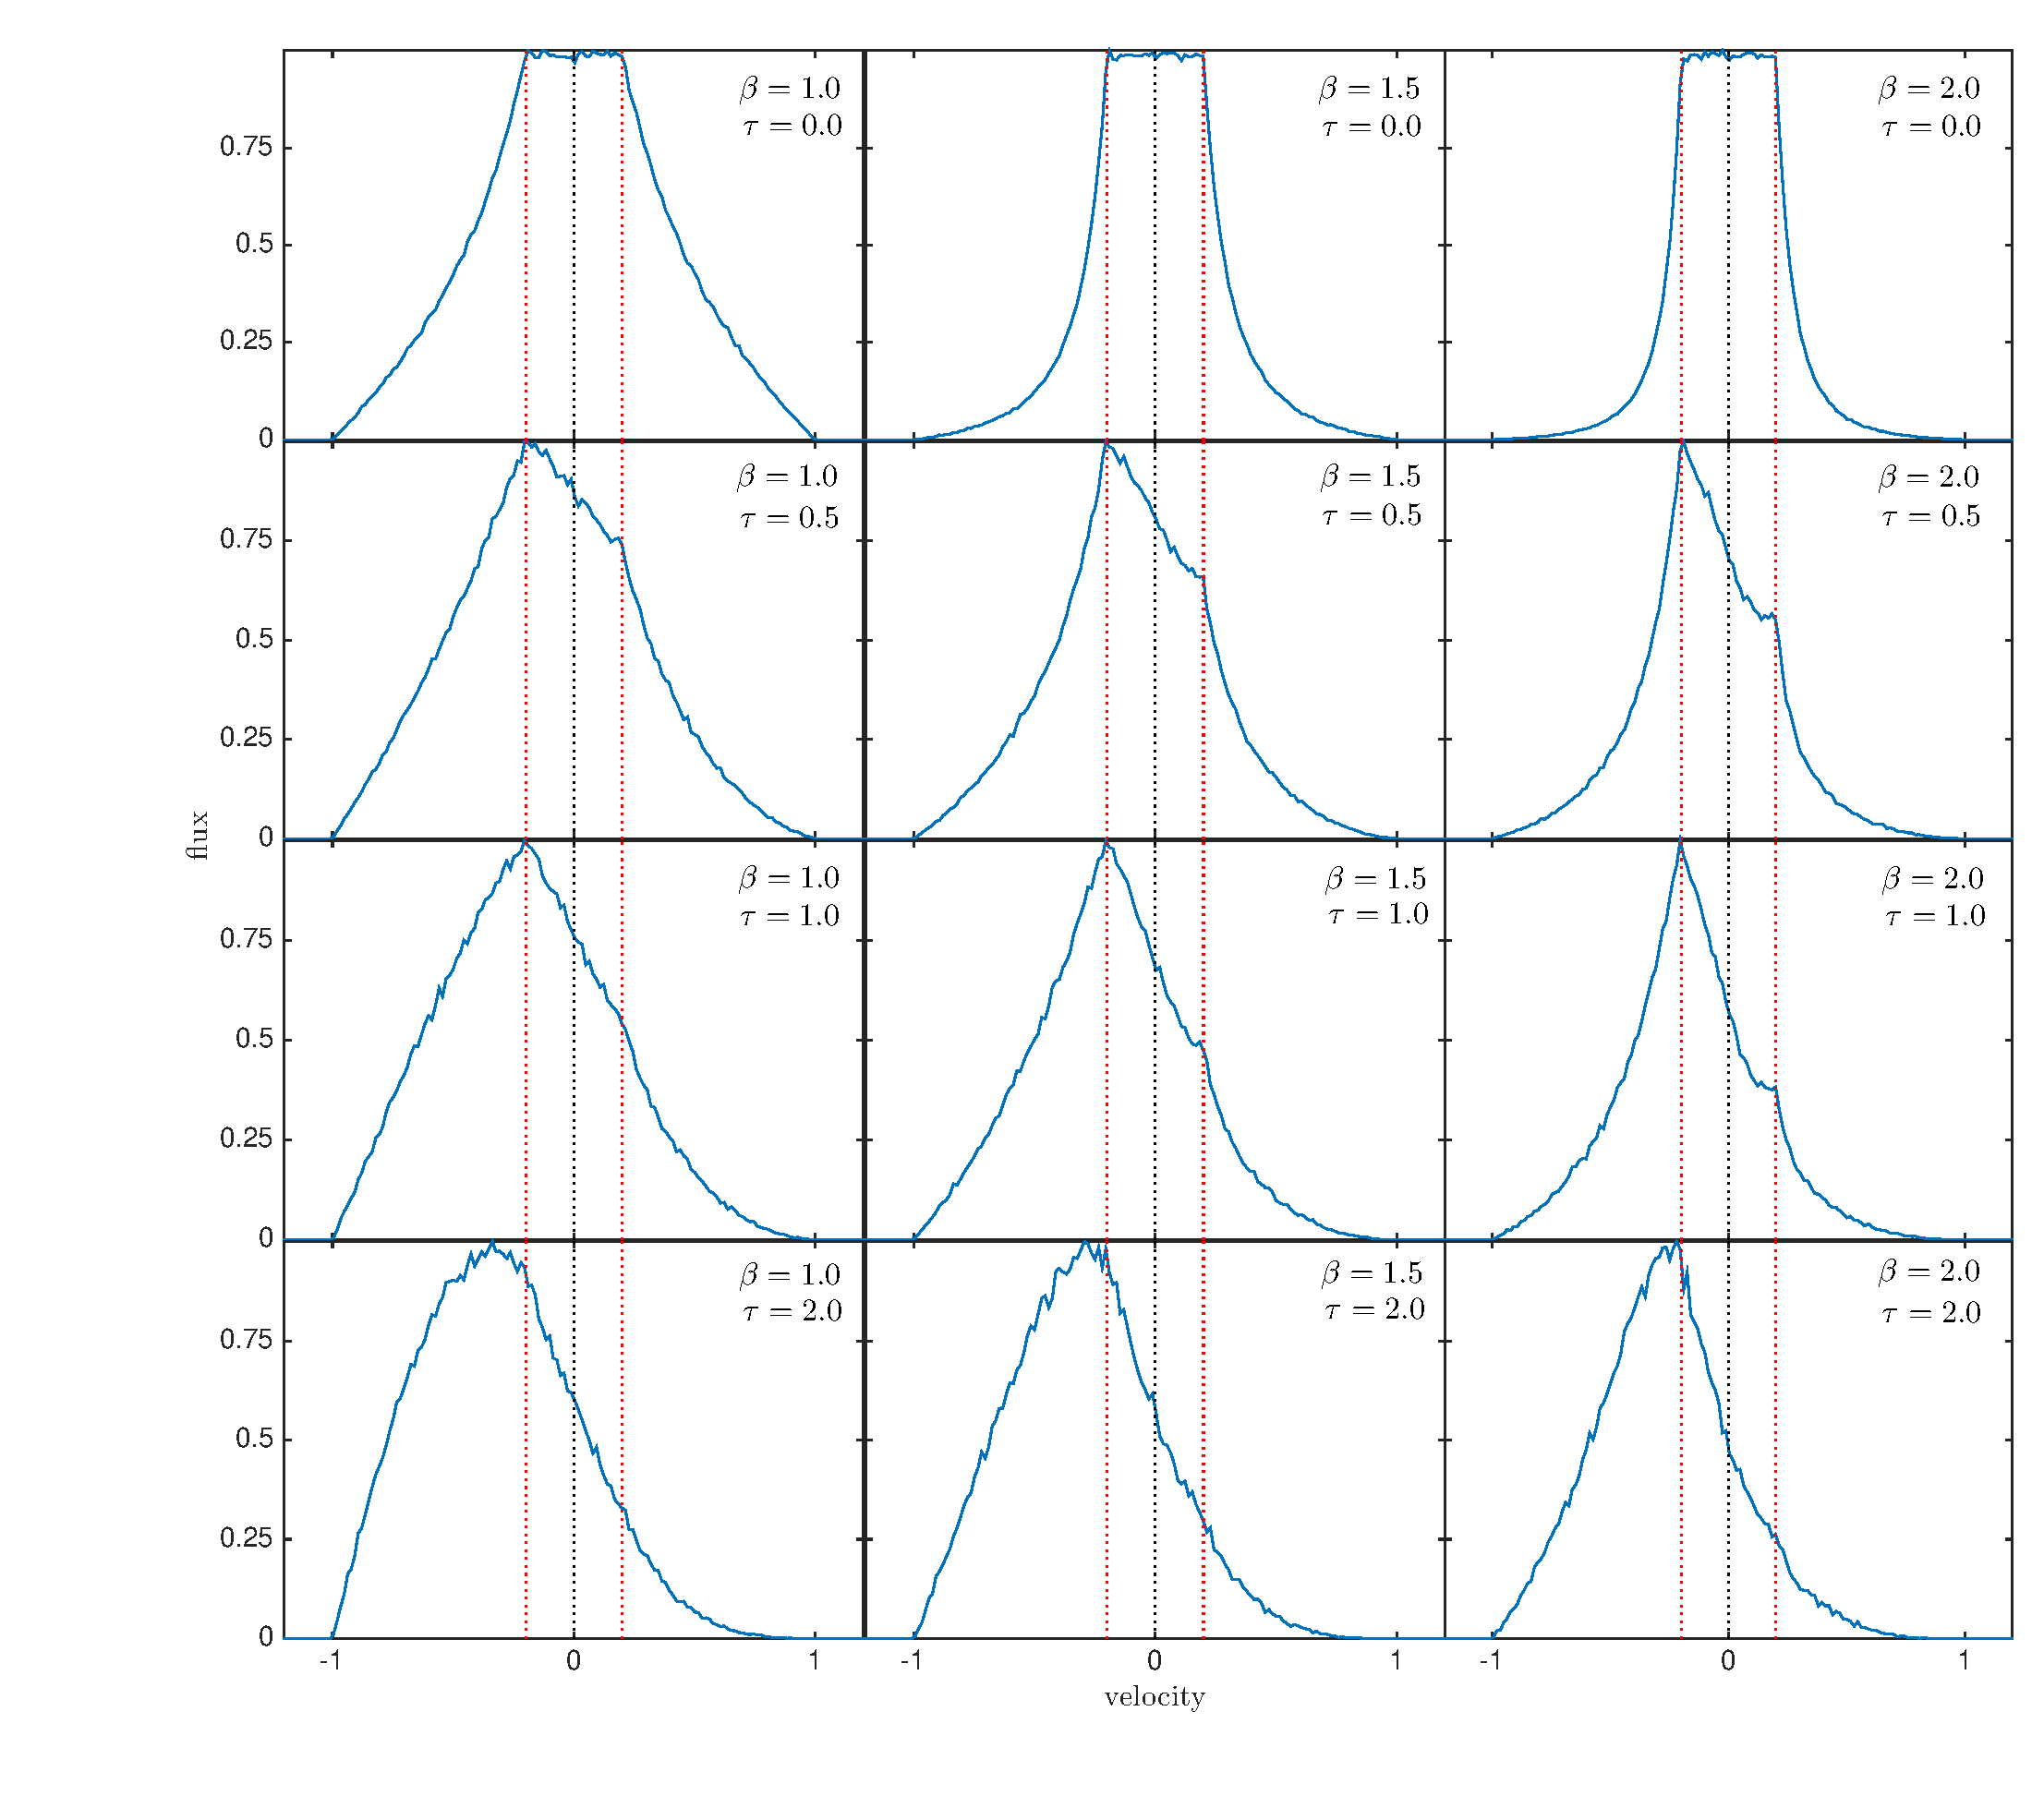
\includegraphics[trim =80 10 6 15,clip=true,scale=0.515]{params/D/newDall} 
\caption{Set of models with $i(r) \propto r^{-2\beta}$, $\omega=0$, 
$R_{in}/R_{out}=0.2$ and $v_{max}=1$ illustrating the effects of varying 
$\tau$ and $\omega$.  Maximum fluxes are scaled to 1.}
\label{bt}
\end{figure*}

\begin{figure*}
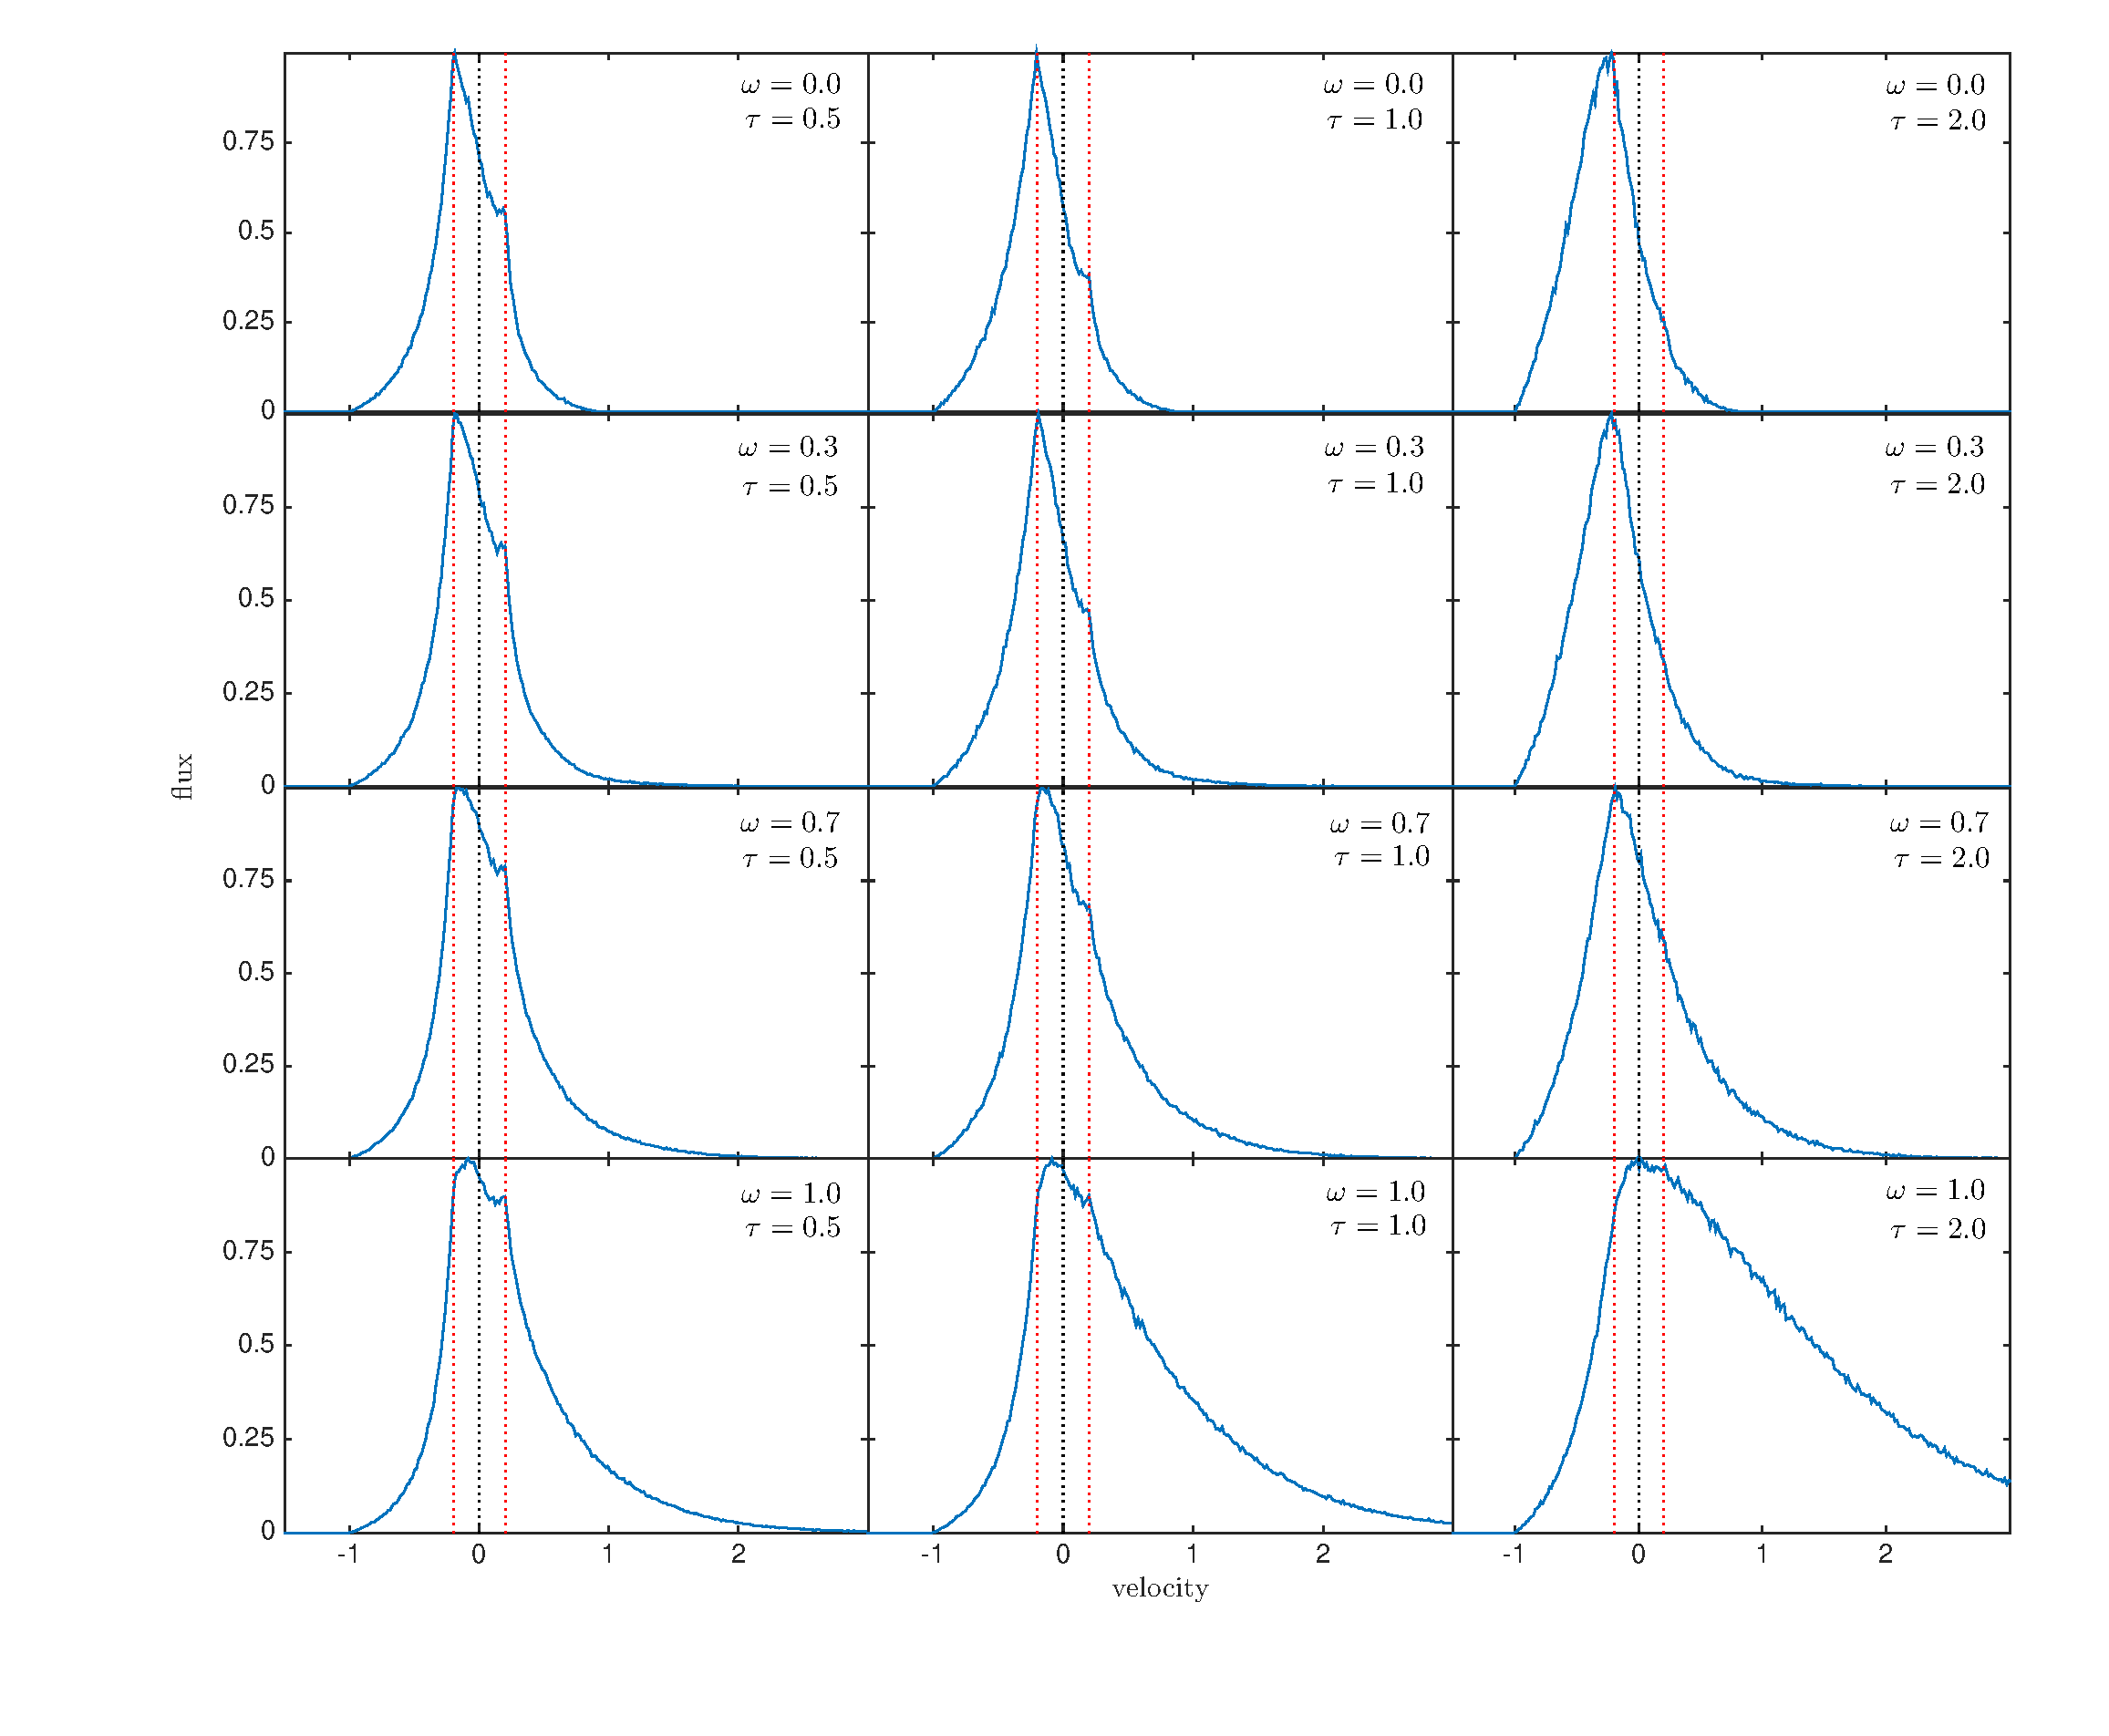
\includegraphics[trim =80 10 40 15,clip=true,scale=0.515]{params/C/C_all} 
\caption{Set of models with $i(r) \propto r^{-4}$, $R_{in}/R_{out}=0.2$ 
and $v_{max}=1$ illustrating the effects of varying $\tau$ and $\omega$. 
Maximum flux is scaled to 1. }
\label{wt}
\end{figure*}


It is of general interest to establish potential diagnostic signatures in 
the profiles of supernovae and their remnants in order to trace dust 
formation more effectively.  We here discuss the effects of the main 
parameters of interest, namely:

\begin{itemize}
\item $v_{max}$
\item $R_{in}/R_{out}$
\item $\beta$, where $\rho \propto r^{-\beta}$
\item albedo $\omega$ 
\item optical depth  $\tau$
\end{itemize}


\subsubsection{$v_{max}$}

The maximum velocity is defined as the velocity at the very outer edges of 
the line emitting region for a given line.  Note therefore that the 
maximum velocity may vary between different spectral lines or doublets due 
to the location of a particular species or differing ionization 
thresholds.  Clearly, the larger the maximum velocity used the wider the 
profile becomes.  To some extent therefore the incline of the density 
profile and the maximum velocity act to counter each other since a steeper 
density profile narrows the profile (see section \ref{beta}).  The shape 
of the wings of the profiles, however, generally preclude much degeneracy 
in this aspect - the overall shape of the line profile determines the 
exponent of the density profile to within a relatively small range.

More important is the effect that the maximum velocity has on the overall 
optical depth.  Since the overall volume of the ejecta is determined 
solely by the maximum velocity and the ratio of the inner and outer radii, 
the total optical depth to which the radiation is exposed is greatly 
affected by even a relatively small change in the maximum velocity.  
Practically speaking, the maximum velocity may be fairly well determined 
from the observations (as identified as the point where the flux vanished 
on the blue side) and may be further constrained through modelling.

\subsubsection{$R_{in}/R_{out}$}

As already discussed in section \ref{analytics}, the width of the flat top 
may be determined solely by the ratio of the inner and outer radii, the 
exponent of the velocity profile and the maximum velocity.  It is valid to 
assume that the velocity profile takes the form $v \propto r$ even from 
just a few months after the explosion as the supernova is in free 
expansion.  This means that $R_{in}/R_{out}$ may be calculated as

\[
\frac{R_{in}}{R_{out}}=\frac{v_{min}}{v_{max}}
\]

\noindent where it is often possible to constrain $v_{min}$ and $v_{max}$ 
to a relatively narrow range simply from the observed line profile.

The majority of spectral lines emitted from supernovae and supernova 
remnants would be expected to have a flat top since it is rare for these 
objects to form a complete nebula.  However, even a very small amount of 
attenuation may result in the profile appearing to be more smoothed at its 
peak.

The effect on the line profile of adopting $R_{in}/R_{out}=0$ as opposed 
to a detached shell may be seen in figure \ref{fig:analytics}.

\subsubsection{$\tau$}
\label{tau}

As expected, greater attenuation of the original line profile is seen on 
the red side than on the blue.  The profiles are most revealing at lower 
optical depths.  The affects of the asymmetric absorption can be seen in 
different sections of the profiles.  The region of the profile that is 
most clearly affected by dust absorption is the flat-topped region.  A 
small amount of absorption in this region results in a skewed profile, 
with a fraction of the flat-topped section removed.  The peak becomes 
blue-shifted as a result, but only to the original value of the minimum 
velocity of the profile. In addition to the attenuation in this region, 
the red wing of the profile is also somewhat reduced, and the blue wing 
somewhat increased relative to their original symmetric positions.  The 
result is a relatively 'jagged' looking profile, often with sharp changes 
at $\pm v_{min}$.  The profile is generally asymmetric, although the 
degree of absorption in the flat-topped region may sometimes make it seem 
as though the profile is in fact symmetric and uniformly blue-shifted (see 
section \ref{asym} for further discussion).

At high optical depths the entire profile is shifted to the blue and the 
peak moves beyond the minimum velocity further into the blue.  The 
profiles also become more smoothed.  A full set of models investigating 
the effects of varying optical depths under different density profiles and 
albedos are presented in figures \ref{bt} and \ref{wt}.

\subsubsection{$\omega$}
\label{omega}

In the past, focus has largely been on the effects of absorption by dust 
on the shapes of line profiles and little attention has been paid to the 
potential effects of scattering by dust grains.  In fact, line profiles 
are significantly affected by scattering of radiation.  Not only does 
repeated scattering of photons increase the number of potential 
opportunities for a given photon to be absorbed but it also results in 
continuous shifting of the frequency of the photon to the red.  The photon 
must do work on the expanding shell of dust in order to escape and thus 
many of the photons are reprocessed beyond the theoretical maximum 
velocity into the red side of the profile.  The result is a substantial, 
extended wing on the red side of the line.  In the case of strong 
scatterers, this can result in an asymmetric profile that is the reverse 
of that normally expected with the majority of the emission on the 
\textit{red} side.  The peak however, remains blue-shifted.  See figure 
\ref{wt} for a full investigation of the variation of $\omega$ and $\tau$.

The implications of this result in relation to the use of line profiles as 
a diagnostic for tracing dust formation in supernova ejecta are 
significant and are discussed further in section \ref{asym}.


\subsubsection{$\rho \propto r^{-2\beta}$}
\label{beta}

Whilst the density profile of the dust may have some effect on the 
resulting profiles, it is the initial emissivity profile (dependent on the 
dust density profile) that has greatest effect on the resulting shape of 
the line profile.

In general, the steeper the emissivity distribution, the narrower the line 
profile becomes.  The sides of the line profile may become almost straight 
for a very steep distribution since the majority of the emission then 
comes from a very narrow velocity range.  For a flat-topped profile of 
fixed width this approximates the square profile produced in the case of 
an emitting shell with constant velocity.

The dependence of the shape of the line profile in the optically thin case 
is described in section \ref{analytics}.  However, the density profile 
also plays a significant role where there is even a small amount of 
absorption.  As previously discussed, at relatively small optical depths, 
a section of the flat-topped region is removed resulting in a peak at 
$-v_{min}$.  The shape of the profile in this region is significantly 
affected by the density profile.  Shallow profiles produce a virtually 
linear variation in flux between $-v_{min}$ and $+v_{min}$.  For a fixed 
optical depth, the steeper the distribution becomes, the more concave the 
profile becomes between $-v_{min}$ and $+v_{min}$, ultimately resulting in 
a clear shoulder to the profile at $+v_{min}$.  For extremely steep 
distributions this ultimately results in a double peaked profile with the 
trough to the red of $v=0$.  A full investigation of the variation of 
$\beta$ with $\tau$ is performed given in figure \ref{bt}.

\subsection{Inferring properties of the dust from the models}

\begin{figure}
\begin{center}
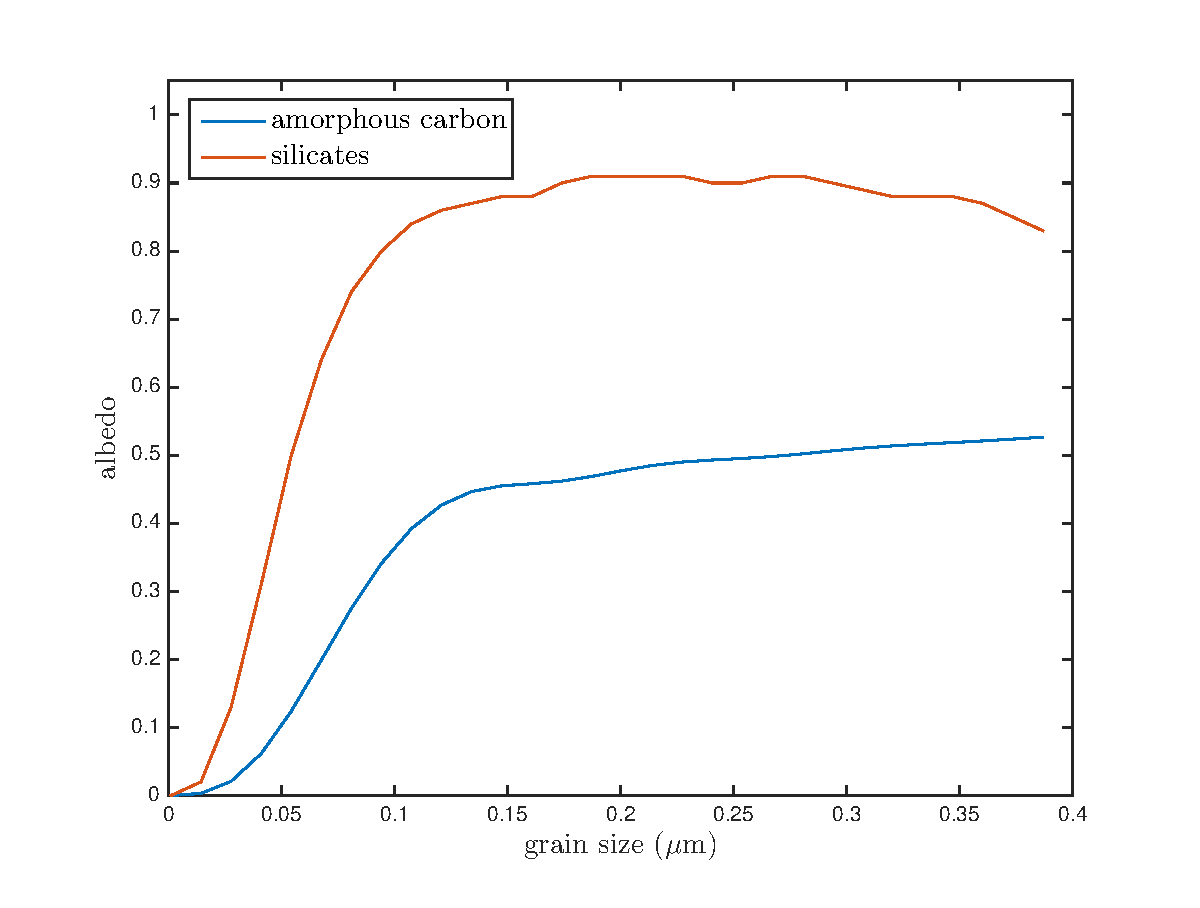
\includegraphics[trim =37 10 45 15,clip=true,scale=0.51]{grainsize_albedo}
\caption{Variation of albedo with grain size for amorpous carbon sample 
using a Mie approximation at $\lambda = 658 \mu $m. Optical constants 
from \citet{Zubko1996}.}
\label{albedo_grain}
\end{center}
\end{figure}

The presence of an extended red wing at large positive velocities in 
combination with increased extinction on this side at smaller positive 
velocities may allow for the values of $\tau$ and $\omega$ to be well 
constrained.  In this case it is possible to translate these values into a 
dust mass and average grain size for a given species or combination of 
species using optical properties and a Mie approximation (see figure 
\ref{albedo_grain}).  In fact, it is the dust mass and average grain size 
that is varied within the code for a specified species or combination of 
species.  It is therefore important to note that the use of different 
optical properties may substantially alter the produced optical depths and 
albedos for a given species of specific grain size as has been noted 
previously \citep{Owen2015}.

\begin{table*}
	\begin{minipage}{180mm}
	\caption{Details of the parameters used for the best fitting smooth models with $a=0.35\mu$m.}
	\label{smooth1}
	\begin{center}
  	\begin{tabular}{@{} ccccccccccccl @{}}
    	\hline
 & day & $v_{max}$ & $R_{in}/R_{out}$ & $\beta$ & $M_{dust}$ & $a$ & $R_{out}$ & $R_{in}$ & doublet ratio & $\tau_{H\alpha}$ & $\tau_V$  & Figure No. \\
	&& (km~s$^{-1} $) & & & ($M_{\odot}$) & ($\mu$m) & (cm) & (cm)  \\
	\hline
H$\alpha$ & 714 & 3250 & 0.25 & 1.2 & 2.50E-05 & 0.35 & 2.00E+16 & 5.01E+15 & & 0.61 & 1.23 &  Fig. \ref{d714bf}\\
H$\alpha$ & 806 & 4500 & 0.25 & 1.8 & 3.00E-05 & 0.35 & 3.13E+16 & 7.83E+15 & & 0.30 & 0.60 &  Fig. \ref{d806bf}\\
H$\alpha$ & 1862 & 8500 & 0.15 & 1.9 & 6.00E-04 & 0.35 & 1.37E+17 & 2.05E+16 & & 0.35 & 0.70 &  Fig. \ref{d1862_3604}\\
H$\alpha$ & 2875 & 9500 & 0.14 & 1.9 & 1.80E-03 & 0.35 & 2.36E+17 & 3.30E+16 & & 0.36 & 0.72 &  Fig. \ref{d1862_3604}\\
H$\alpha$ & 3604 & 10250 & 0.13 & 1.9 & 5.00E-03 & 0.35 & 3.19E+17 & 4.15E+16 & & 0.55 & 1.10 &  Fig. \ref{d1862_3604}\\ \relax
[O~{\sc i}]  & 714 & 5000 & 0.17 & 2.8 & 9.50E-05 & 0.35 & 3.08E+16 & 5.24E+15 & 2.9 & 1.09 & 2.19 & Fig. \ref{d714bf}\\ \relax
[O~{\sc i}]  & 806 & 6000 & 0.15 & 2.7 & 1.60E-04 & 0.35 & 4.18E+16 & 6.27E+15 & 2.7 & 0.97 & 1.95 & Fig. \ref{d806bf} \\
    \hline
  \end{tabular}
  \end{center}
\end{minipage}
\end{table*}

For amorphous carbon, the larger the grain size used the larger the albedo 
and the smaller the cross-section of absorption.  Larger masses of dust 
are therefore required to fit the same degree of absorption if a larger 
grain size is used.  This is in contrast to SED radiative transfer 
modelling where larger grain sizes generally result in less dust being 
required to fit the IR portion of the SED (W15).  These two techniques in 
tandem may therefore give excellent limits on grain sizes for specific 
species or combinations thereof.


\subsection{Observable signatures of dust in line profiles}
\label{asym}

The greater the optical depth modelled, the more attenuation of the line 
is observed.  As expected, the blue side of the profile suffers a greater 
degree of absorption than the red side.  The resulting asymmetry is 
somewhat more complex than perhaps previously thought however.  Dust has 
repeatedly been cited as the agent responsible for the apparent 
blue-shifting of line profiles in supernovae in the manner of the profiles 
presented in figure \ref{fig:Lucy}.  That is, relatively high optical 
depths result in an overall shift of the entire profile towards the blue.

In practice a relatively large optical depth ($\tau \approx 2$) is 
required to actively shift the peak of the profile beyond its natural 
minimum velocity.  In most cases it seems more likely that the medium is 
in fact optically thin and the blue-shifting of the peak of the profile is 
likely a result of attenuation in the flat-topped section (close to 
$R_{in}$).  The peak would therefore be located at $-v_{min}$.

Dust absorption is wavelength dependent.  One might therefore expect the 
position of the peak to be dependent on the wavelength of the line being 
considered.  Indeed, the relationship between the locations of the peaks 
of profiles and their wavelength has been discussed by several authors in 
relation to dust formation \citep{Gall2014,Fransson2013,Smith2012}.  We 
suggest here, that whilst this is likely the case in regions of high 
optical depth, this is not necessarily likely to be seen in the ejecta of 
most supernovae.  The wavelength-dependence of dust absorption instead 
results in differing degrees of extinction in the flat-topped region of 
each profile but leaves the peak at its blue-shifted position of 
$-v_{min}$.  Of course, the value of $v_{min}$ may be different for 
different species.  However, if this is the case then there would be no 
reason to expect variation in the position of the peaks of profile to be 
correlated with the wavelength dependence of dust.  Rather one would it 
expect it potentially to trace the location of elements within the ejecta.


The attenuation of the flat-topped region is also often such that it may 
be very hard to discern a difference in slope between the attenuated 
section between $-v_{min}$ and $+v_{min}$ and the slope of the wing for 
$v>+v_{min}$, particularly in circumstances where data is of poor 
resolution or has a poor signal-to-noise ratio.  Even in the case of 
excellent data, it may be easy to overlook these particular features or to 
dismiss them as natural fluctuations in the geometry of the ejecta.  The 
possibility that they may be a product of dust formation should be 
considered.

The greater attenuation of radiation received from the receding portion of 
the ejecta results in an asymmetry of the line profile whereby the 
majority of emission is contained bluewards of the peak.  However, there 
is an extent to which the effects of repeated scattering events within the 
ejecta serves to counter this asymmetry.  Even in the case of dust grains 
with a relatively low albedo, a surprisingly persistent wing on the red 
side of the profile is seen, often beyond the maximum theoretical velocity 
of the emitting region.  For higher albedos this can actively result in a 
shift in the overall asymmetry of the profile, with the majority of the 
emission being emitted redwards of the peak, though the peak itself 
remains blue-shifted.

This effect is obviously analogous to that of electron scattering which 
also produces a significant red wing in line profiles \citep{Hillier1991, 
Auer1972b}. This is an important consideration in both modelling and 
analysis of spectral line profiles.  DAMOCLES has the capacity to include 
a basic electron scattering mechanism in order to assess the possibility 
that any observed red wing might be produced by electron scattering rather 
than dust scattering.  The red wing observed in line profiles is an 
excellent diagnostic for determining the overall albedo and it is 
therefore important to establish whether the origins of this feature are 
electron or dust scattering or a combination of the two.

The combination of relatively low optical depths, initially flat-topped 
profiles, greater attenuation on the blue side with increased flux on the 
red side due to scattering results in a profile that, somewhat bizarrely, 
can often end up appearing almost symmetrical, particularly if 
contaminants such as narrow lines or blending with other broad lines are 
present or if the resolution of the data is poor.  Obviously highly 
asymmetrical profiles are also observed, but the potential for apparently 
symmetrical profiles that appear to have been uniformly blue-shifted 
should be noted and analysed carefully (see figures \ref{bt} and \ref{wt} 
for examples of this).


\section{Results}
\label{results}

\begin{figure}
\begin{center}
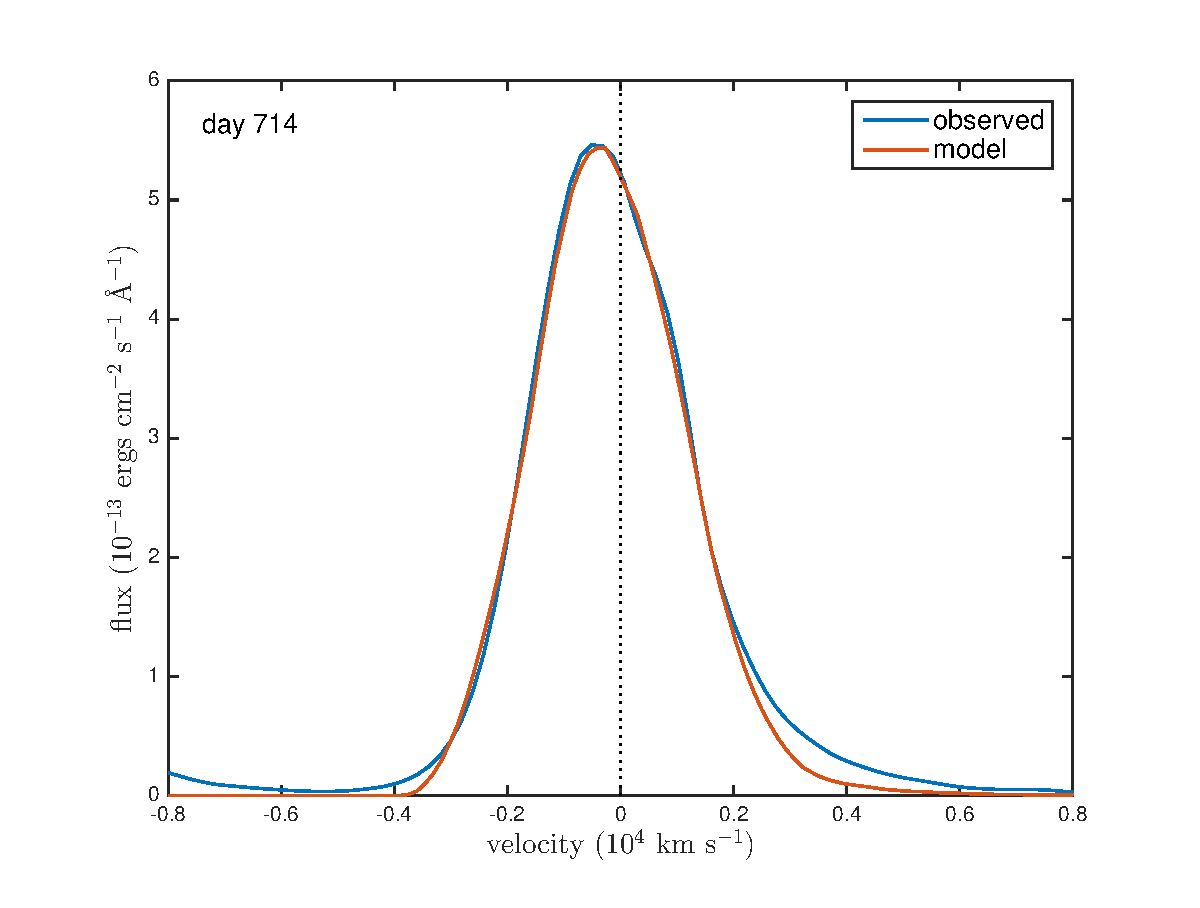
\includegraphics[trim =37 10 45 15,clip=true,scale=0.51]{smooth/d714Ha_smooth_amC_MRN}
\caption{Conservative fit to the day 714 H$\alpha$ line illustrating the 
underestimation of the red scattering wing for small grain sizes.  Model 
parameters are the same as the conservative fit to day 714 except for the 
grain size distribution and dust mass:  $v_{max}=3250$ km~s$^{-1}$, 
$R_{in}/R_{out}$=0.25, $\beta = 1.2$, $M_{dust}=8.0 \times 10^{-6} 
M_{\odot}$, $a_{min}=0.005 \mu$m, $a_{max}=0.25 \mu$m and $n(a) \propto 
a^{-3.5}$.}
\label{MRN}
\end{center}
\end{figure}

\begin{figure*}
\begin{center}
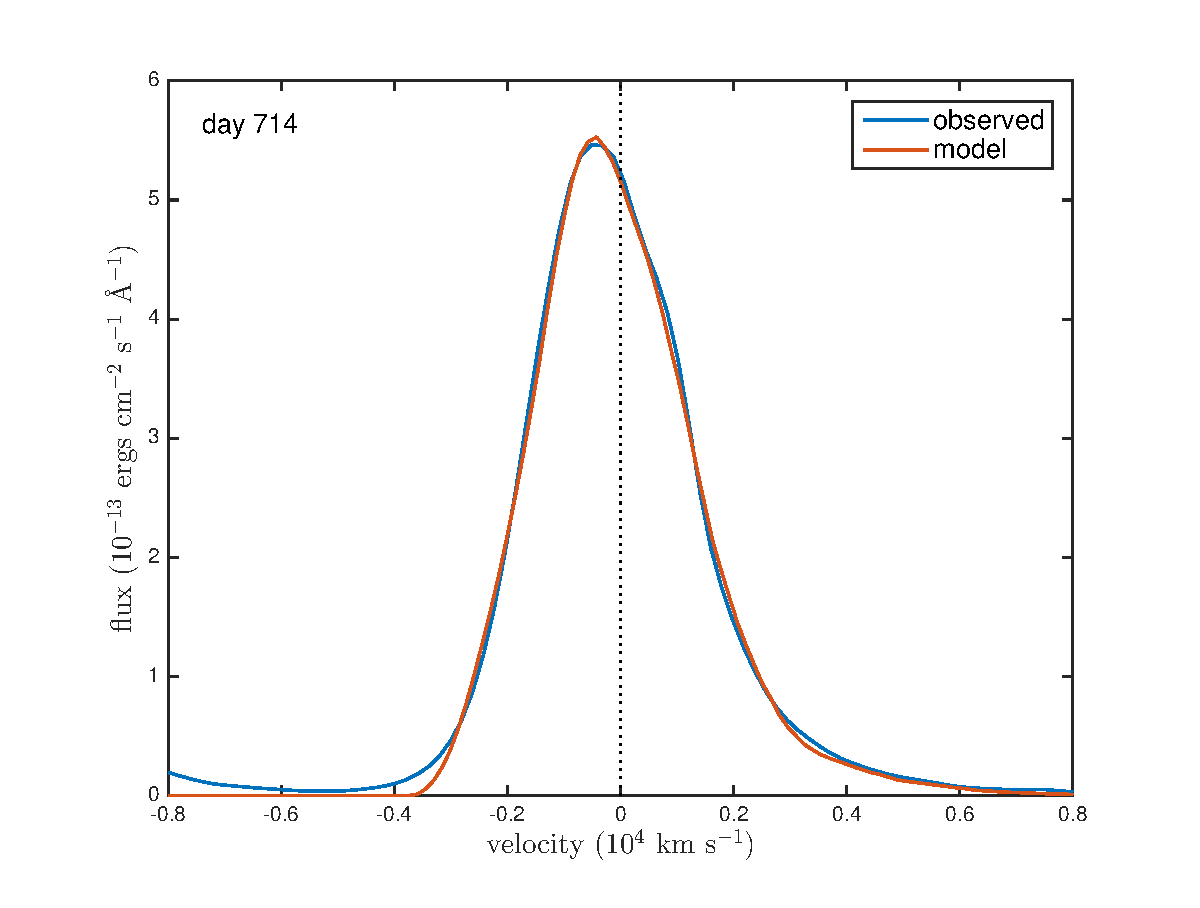
\includegraphics[trim =37 10 45 15,clip=true,scale=0.51]{smooth/best_fit/d714Ha}
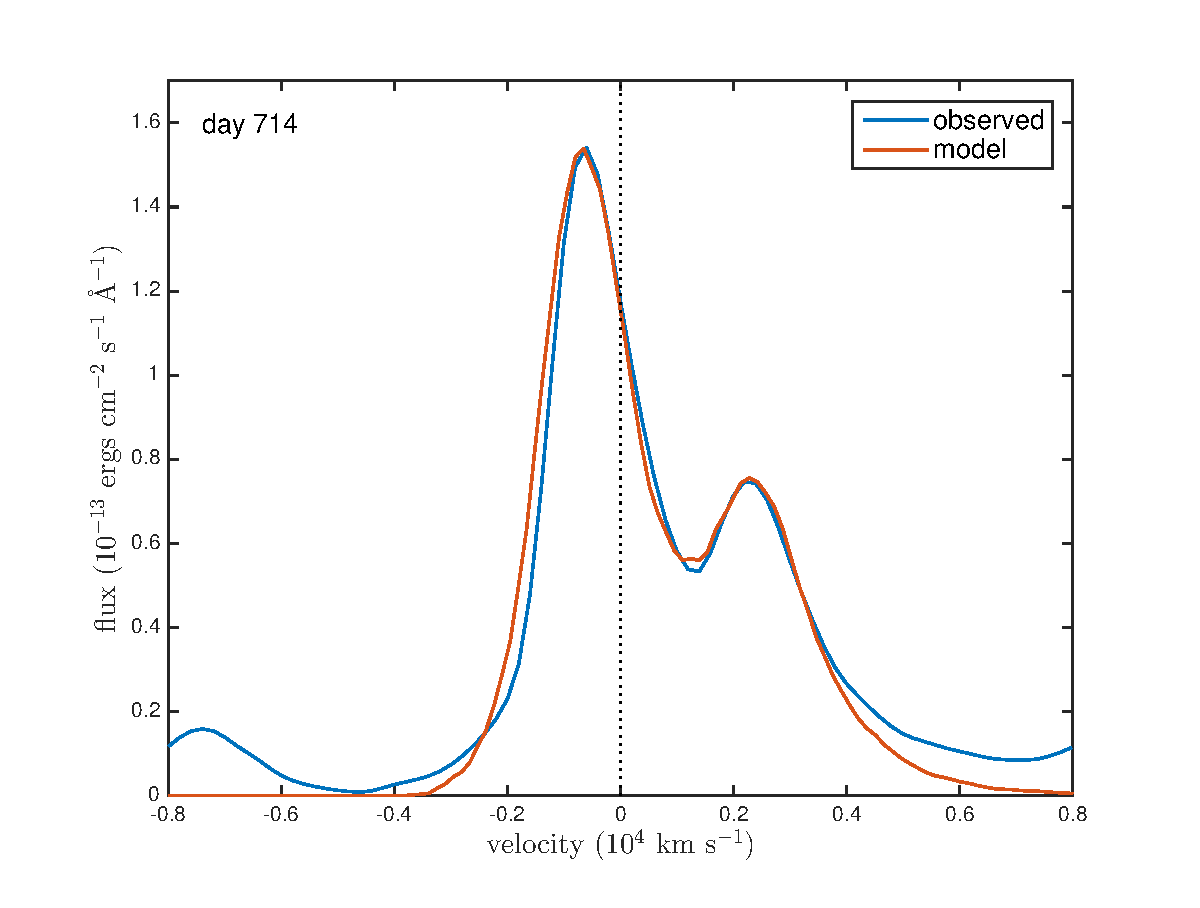
\includegraphics[trim =37 10 45 15,clip=true,scale=0.51]{smooth/best_fit/d714OI}
\caption{Best smooth fit to the day 714 H$\alpha$ line (left) and 
[O~{\sc i}] $\lambda$6300,6363~\AA\ doublet (right) as per parameters 
detailed in table \ref{smooth1}.}
\label{d714bf}
\end{center}
\end{figure*}
\begin{figure*}
\begin{center}
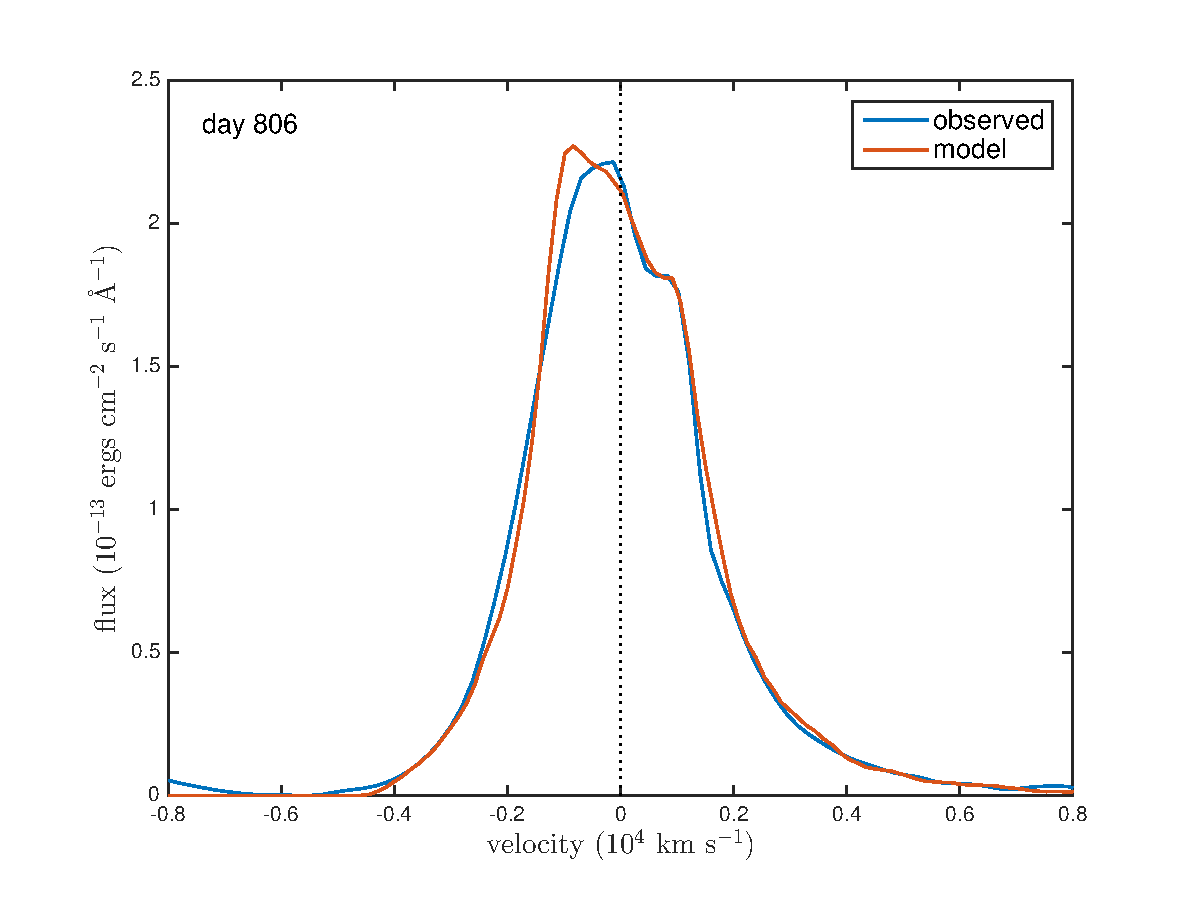
\includegraphics[trim =37 10 45 15,clip=true,scale=0.51]{smooth/best_fit/d806Ha}
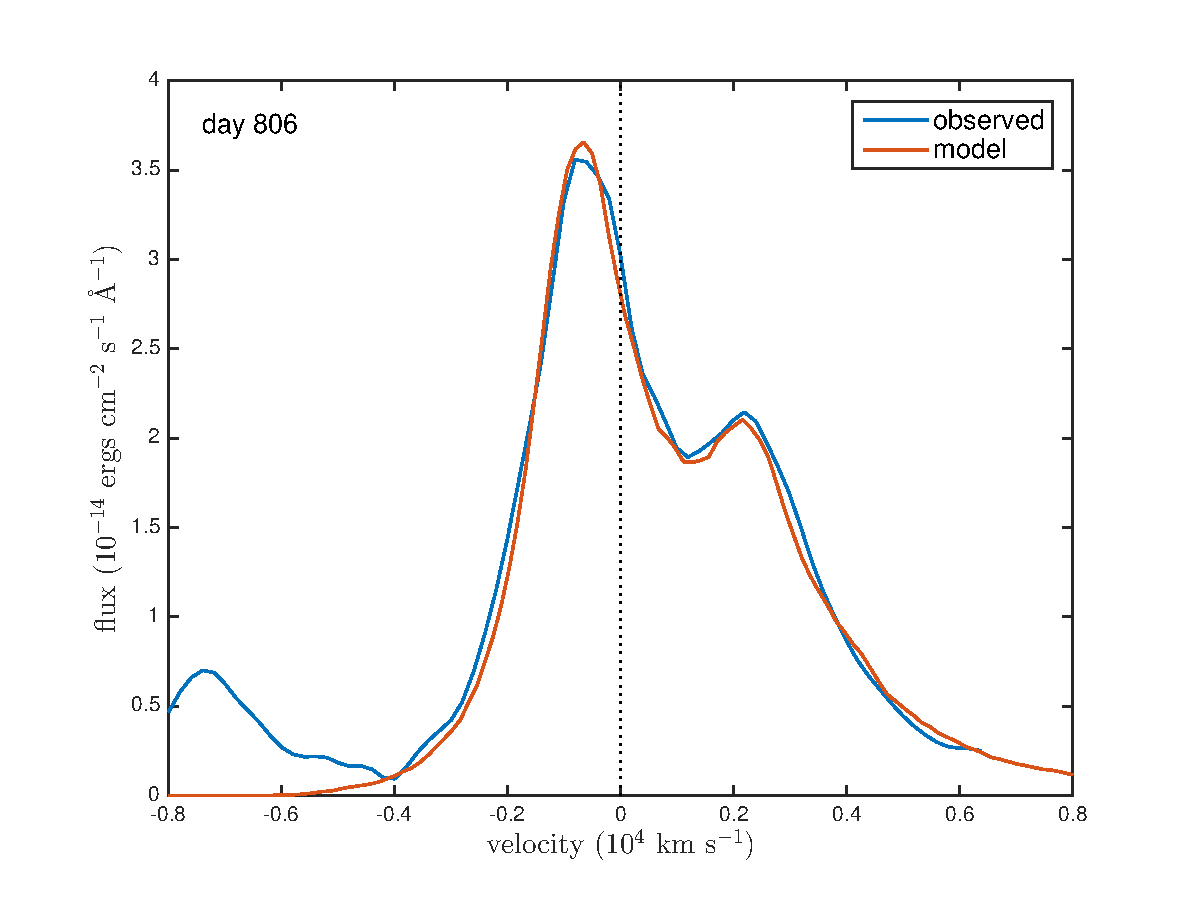
\includegraphics[trim =37 10 45 15,clip=true,scale=0.51]{smooth/best_fit/d806OI}
\caption{Best smooth fit to the day 806 H$\alpha$ line (left) and the 
[O~{\sc i}] $\lambda$6300,6363~\AA\ doublet (right) as per parameters 
detailed in Table \ref{smooth1}.}
\label{d806bf}
\end{center}
\end{figure*}


We model the H$\alpha$ line at days 714, 806, 1862, 2875 and 3604 and the 
[O~{\sc i}] $\lambda$6300,6363~\AA\ doublet at days 714 and 806. After this 
epoch the profile begins to become dominated by emission from the reverse shock 
and the structure of the emitting region may no longer be approximated by 
a single shell model as we do here.  We maintain a velocity profile $v = 
\frac{v_{max}}{R_{max}}r$ and treat the variable parameters listed in 
section \ref{ps}.  Whilst the albedo and optical depth are not varied 
directly, they are altered by adjusting the dust mass, $M_{dust}$, and the 
grain size, $a$, which will together determine the albedo and optical 
depth via a Mie scattering approximation and the optical properties of the 
dust.

In all models, the ejecta occupies a shell with inner radius $R_{in}$ and 
outer radius $R_{out}$.  Packets are emitted according to a smooth density 
profile assuming recombination such that $i(r) \propto \rho(r)^2 \propto 
r^{-2\beta}$.  Initially the dust is considered to have a smooth density 
distribution and is assumed to be coupled to the gas following the same 
radial profile.  A clumped distribution of dust is considered later (see 
section \ref{clumped_models}).  We do not include electron scattering in 
the code since the electron density is not high enough to affect the line 
profiles in any discernible fashion \textit{references}.

\begin{table*}
	\begin{minipage}{180mm}
	\caption{Details of the parameters used for the best fitting clumped models with $a=0.6\mu$m.}
	\label{clumped1}
	\begin{center}
  	\begin{tabular}{@{} ccccccccccccl @{}}
    	\hline
 & day & $v_{max}$ & $R_{in}/R_{out}$ & $\beta$ & $M_{dust}$ & $a$ & $R_{out}$ & $R_{in}$ &  doublet ratio & $\tau_{H\alpha}$ & $\tau_V$  & Figure No. \\
	&& (km~s$^{-1} $) & & & ($M_{\odot}$) & ($\mu$m) & (cm) & (cm)  \\
	\hline
H$\alpha$ & 714 & 3250 & 0.25 & 1.2 & 7.00E-05 & 0.6 & 2.00E+16 & 5.01E+15 & & 0.87 & 1.74 & Fig. \ref{d714_c} \\
H$\alpha$ & 806 & 4250 & 0.25 & 1.9 & 1.00E-04 & 0.6 & 2.96E+16 & 7.40E+15 & & 0.56 & 1.12 & Fig. \ref{d806_c}\\
H$\alpha$ & 1862 & 8500 & 0.14 & 1.9 & 1.65E-03 & 0.6 & 1.37E+17 & 1.91E+16 & & 0.48 & 0.96 & Fig. \ref{d1862_3604_c}\\
H$\alpha$ & 2875 & 9500 & 0.12 & 2 & 1.00E-02 & 0.6 & 2.36E+17 & 2.83E+16 & & 0.96 & 1.93 & Fig. \ref{d1862_3604_c}\\
H$\alpha$ & 3604 & 10250 & 0.12 & 2 & 2.30E-02 & 0.6 & 3.19E+17 & 3.83E+16 & & 1.21 & 2.42 & Fig. \ref{d1862_3604_c}\\ \relax
[O~{\sc i}]  & 714 & 5000 & 0.17 & 2.8 & 2.70E-04 & 0.6 & 3.08E+16 & 5.24E+15 & 2.6 &  1.02 & 2.03 & Fig. \ref{d714_c}\\ \relax
[O~{\sc i}]  & 806 & 6000 & 0.15 & 2.7 & 6.00E-04 & 0.6 & 4.18E+16 & 6.27E+15 & 2.4 & 1.66 & 3.32 & Fig. \ref{d806_c}\\
    \hline
  \end{tabular}
  \end{center}
\end{minipage}
\end{table*}

\begin{figure*}
\begin{center}
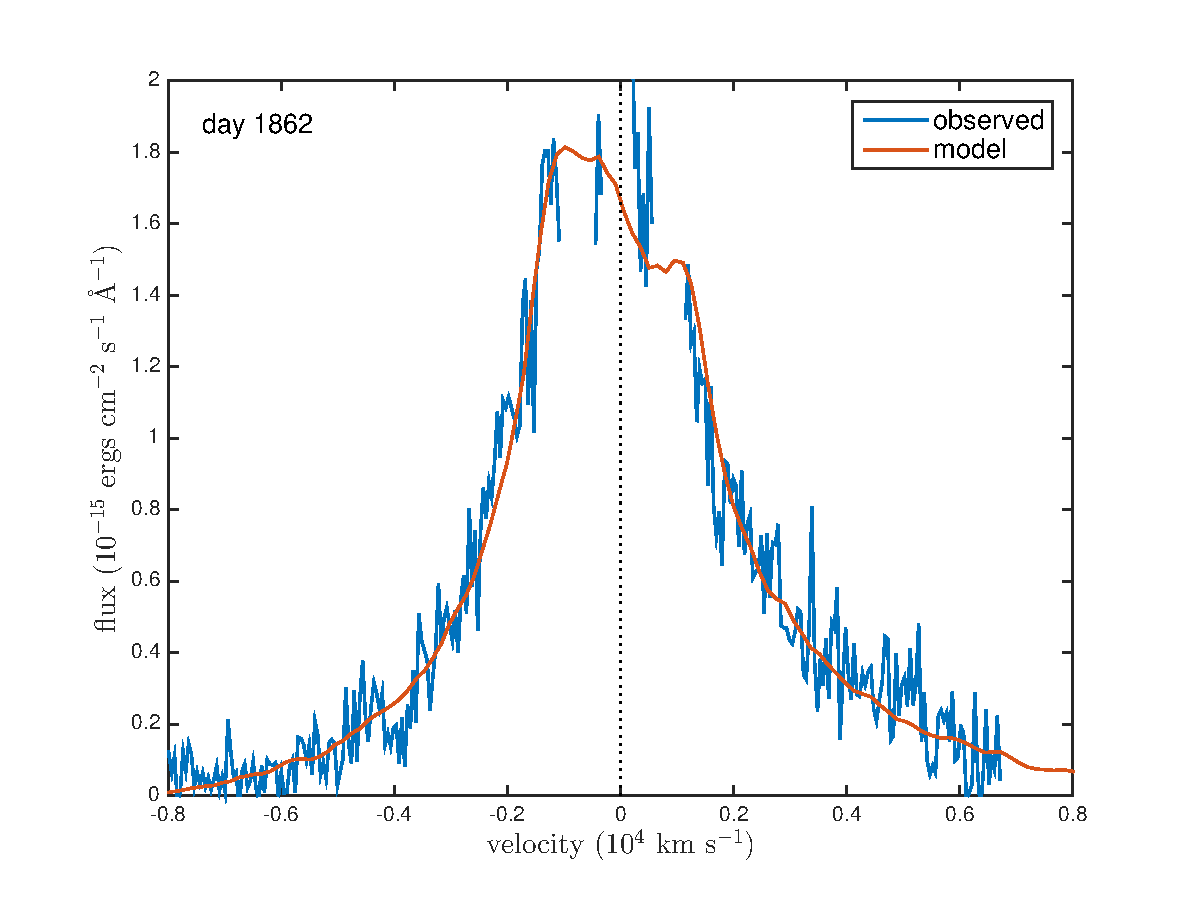
\includegraphics[trim =37 10 45 15,clip=true,scale=0.35]{smooth/best_fit/d1862Ha}
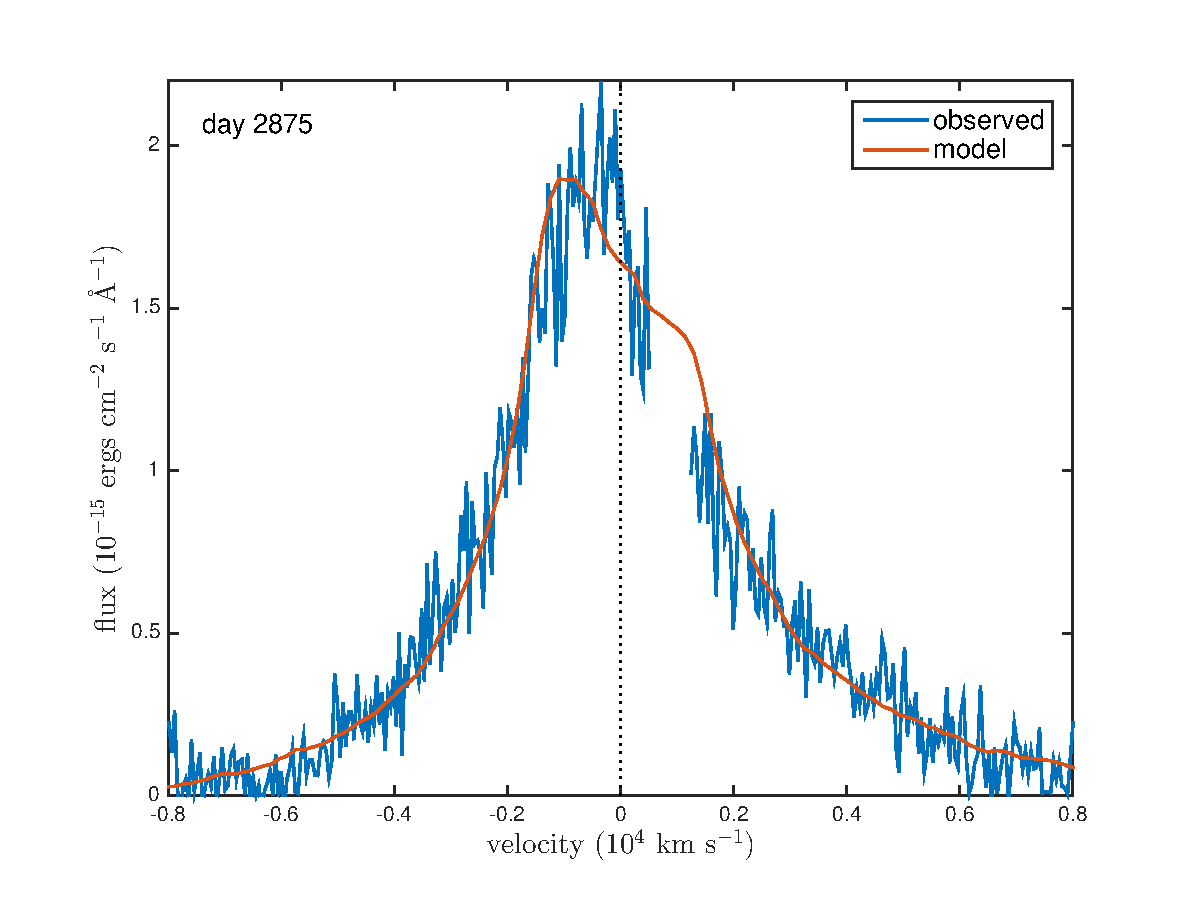
\includegraphics[trim =55 10 45 15,clip=true,scale=0.35]{smooth/best_fit/d2875Ha}
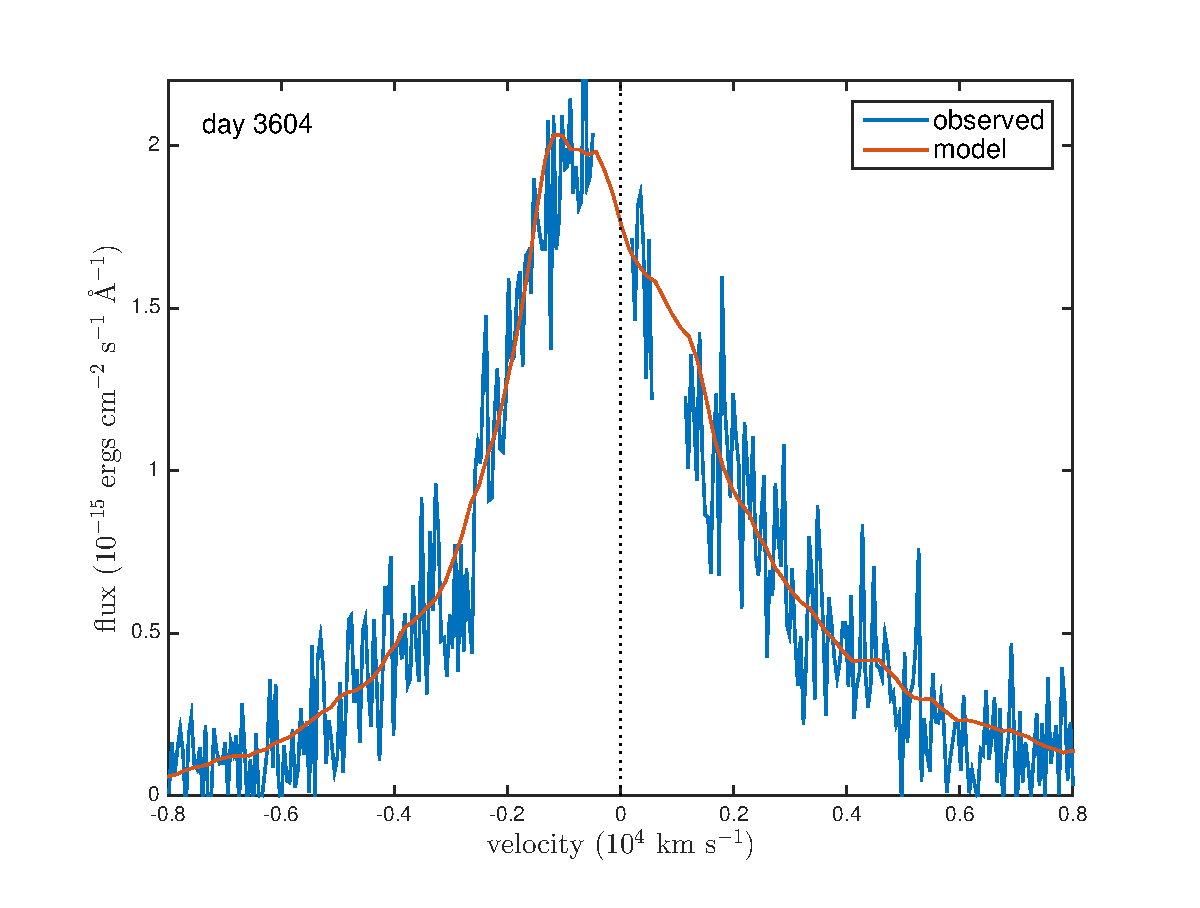
\includegraphics[trim =55 10 45 15,clip=true,scale=0.35]{smooth/best_fit/d3604Ha}
\caption{Best smooth fit to the H$\alpha$ line at days 1862, 2875 and 
3604 as per parameters detailed in table \ref{smooth1}.}
\label{d1862_3604}
\end{center}
\end{figure*}


As might be expected when fitting a single line with many variables, there 
is rarely a unique set of parameters that best fit the data.  However, the 
majority of the parameters of interest may be well constrained by our 
modelling by considering different elements of the shape of the profile as 
we have previously discussed.  In particular, by constructing good fits to 
the data using both conservative and optimistic estimates of the grain 
size, credible lower and upper bounds on the possible dust mass formed 
within the ejecta may be derived.  We therefore present here a number of 
reasonable fits to the data using both small and large values of $a$ since 
it is the grain size which has the most significant effect on the overall 
dust mass required to reproduce the profile (see section \ref{params}).  
We use an environment of pure amorphous carbon and use the optical 
constants from the BE sample presented in \citet{Zubko1996}.  Previous 
modelling has limited the fraction of silicates present in the dusty 
medium to a maximum of 15\% \citep{Wesson2015,Ercolano2007} and so an 
environment of pure amorphous carbon is likely to be reasonably 
representative of the true composition.  If anything, pure amorphous 
carbon is the most conservative choice since the inclusion of even a small 
fraction of silicates is likely to increase the dust mass required.

For each profile, the maximum velocity is identified from the data as the 
point where the flux vanishes on the blue side.  The equivalent point on 
the red side is indeterminate from observations due to the effects of 
scattering.  Similarly, the 'corner' of the flat topped section of the 
profile on the blue side allows the minimum velocity at $R_{in}$ to be 
ascertained. As discussed in section \ref{params}, this allows the ratio 
of the bounds of the supernova to be determined as 
$R_{in}/R_{out}=v_{min}/v_{max}$.  The outer radius is calculated from the 
epoch and maximum velocity.

The only parameters that then remain to be determined are the exponent of 
the density profile $\beta$, the grain size and the dust mass.  The shape 
of the blue wing is solely a product of the density profile and the dust 
mass; the height and shape of the red wing is a product of these and also 
of the scattering efficiency of the grains (the albedo $\omega$); and the 
extent and shape of the asymmetry in the flat-topped portion of the 
profile is a result of only the total optical depth as determined by the 
dust mass and the grain size.  By iterating over these three parameters 
therefore, an excellent fit to the data may be obtained.

Models are produced in the same manner for the [O~{\sc i}] 
$\lambda$6300,6363~\AA\ doublet as for a single line with each component 
of the doublet being modelled independently and the resulting profiles 
added according to a specified ratio.  Although the flux ratio is 
theoretically determined, the actual ratio between the two components is 
affected by self-absorption \textit{reference} and it is therefore 
necessary to leave this as a free parameter.  The [O~{\sc i}] 
$\lambda$6300,6363~\AA\ exhibits a clear blueshift as early as day 611 
and provides another diagnostic for determining the dust mass allowing 
the wavelength dependence of dust absorption to be probed.  By day 1862 
the doublet is too blended and no longer strong enough to usefully 
model.


\subsection{Smooth Models of SN 1987A}
\label{smooth_models}

Even at the earliest epochs there is a substantial wing on the red side of 
the data that cannot be fitted with grains with a small albedo.  The 
minimum required albedo is approximately $\omega \approx 0.5$.  The larger 
the grain size the larger the mass of dust required to reproduce the same 
optical depth (since the optical depth is dependent only on the 
cross-sectional area of the grains).  Figure \ref{MRN} illustrates the 
best fit at day 714 in the case where the classical MRN grain size 
distribution is adopted with $a_{min}=0.005 \mu m$, $a_{max}=0.25 \mu m$ 
and $n(a) \propto a^{-3.5}$.  It can be seen clearly that the red wing is 
significantly underestimated.  Since the scattering efficiency of pure 
amorphous carbon varies significantly over a relatively small grain size 
range (see figure \ref{albedo_grain}) we can establish a reasonably strong 
lower bound on the mean dust grain size, which we estimate to be 
approximately $a=0.35\mu$m.  This is the smallest grain size that is still 
capable of reproducing the red scattering wing at all epochs and we 
therefore use this value throughout our smooth modelling.

The inner and outer radii are calculated at each epoch from the maximum 
velocity used, the day number and the specified ratio $R_{in}/R_{out}$.  
The radii generated are consistent with those used in previous models of 
SN 1987A \citep{Wesson2015,Ercolano2007}.  Figures \ref{d714bf} to 
\ref{d1862_3604} show the best fits to the data for days 714 to 3604 and 
table \ref{smooth1} details the parameters used.

It can be seen that, in order to reproduce the blueshifts seen in the 
[O~{\sc i}] $\lambda$6300,6363~\AA\ doublet, considerably larger dust masses 
are required than to fit the H$\alpha$ line.  However, larger maximum 
velocities are also required to fit the wings and a significantly steeper 
density profile is required.  The inner radii remain approximately similar 
in both the H$\alpha$ and [O~{\sc i}] $\lambda$6300,6363~\AA\ models whilst the 
outer radii are significantly different.  This may indicate why a greater 
dust mass is required in order to fit the [O~{\sc i}] doublet; the doublet 
traces the dust to a wider radius than the H$\alpha$ line.


 \begin{figure*}
\begin{center}
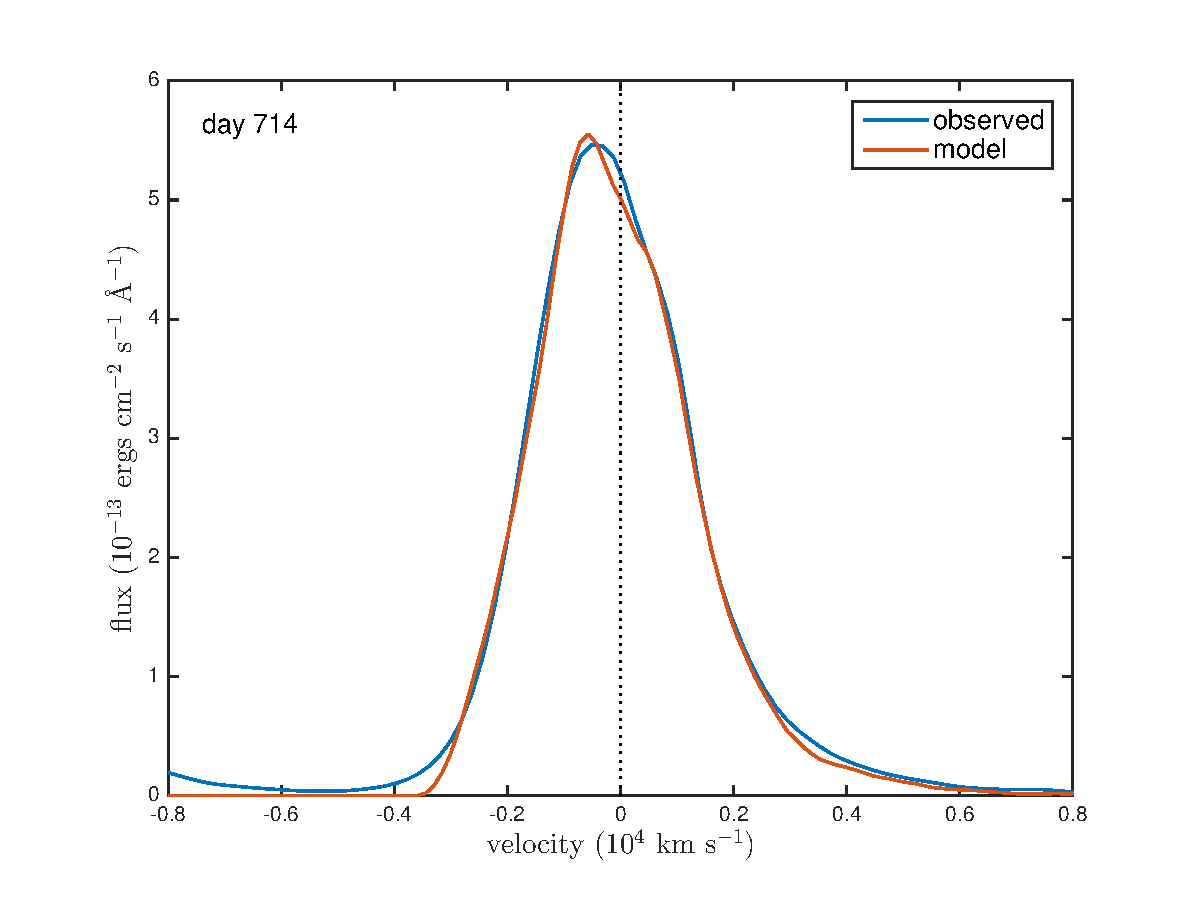
\includegraphics[trim =37 10 45 15,clip=true,scale=0.51]{clump_1/best_fit/d714Ha}
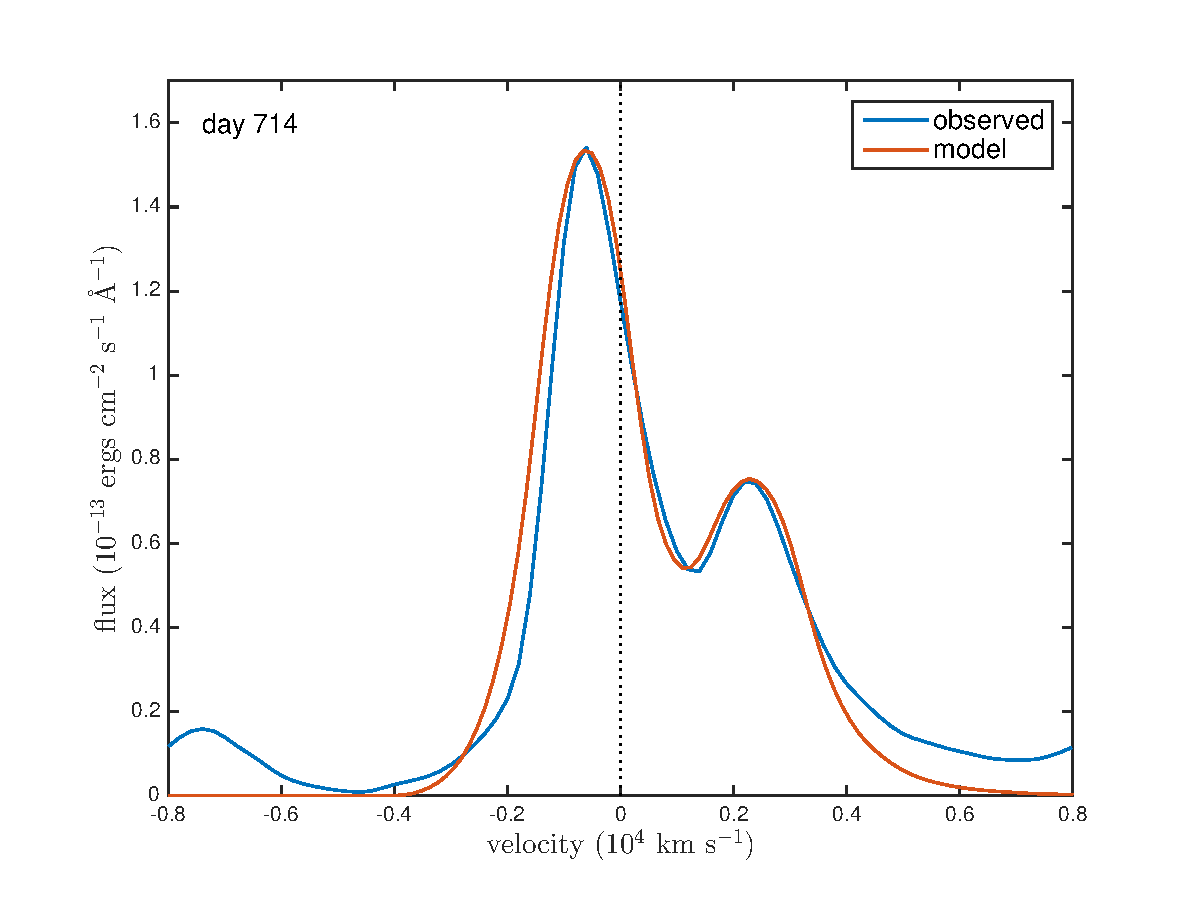
\includegraphics[trim =37 10 45 15,clip=true,scale=0.51]{clump_1/best_fit/d714OI}
\caption{Best clumped fit to the day 714 H$\alpha$ line and [O~{\sc i}] 
$\lambda$6300,6363~\AA\ doublet as per parameters detailed in 
Table \ref{clumped1}.}
\label{d714_c}
\end{center}
\end{figure*}
\begin{figure*}
\begin{center}
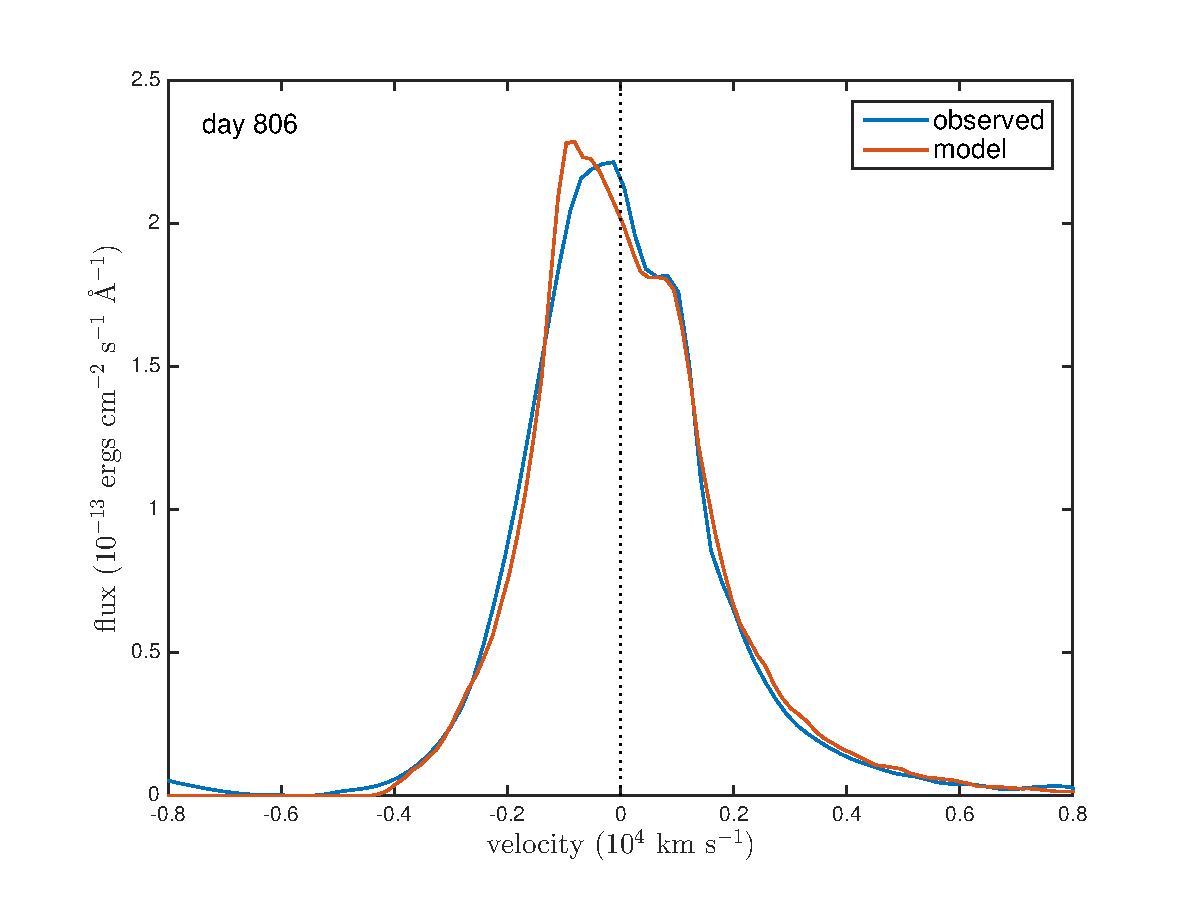
\includegraphics[trim =37 10 45 15,clip=true,scale=0.51]{clump_1/best_fit/d806Ha}
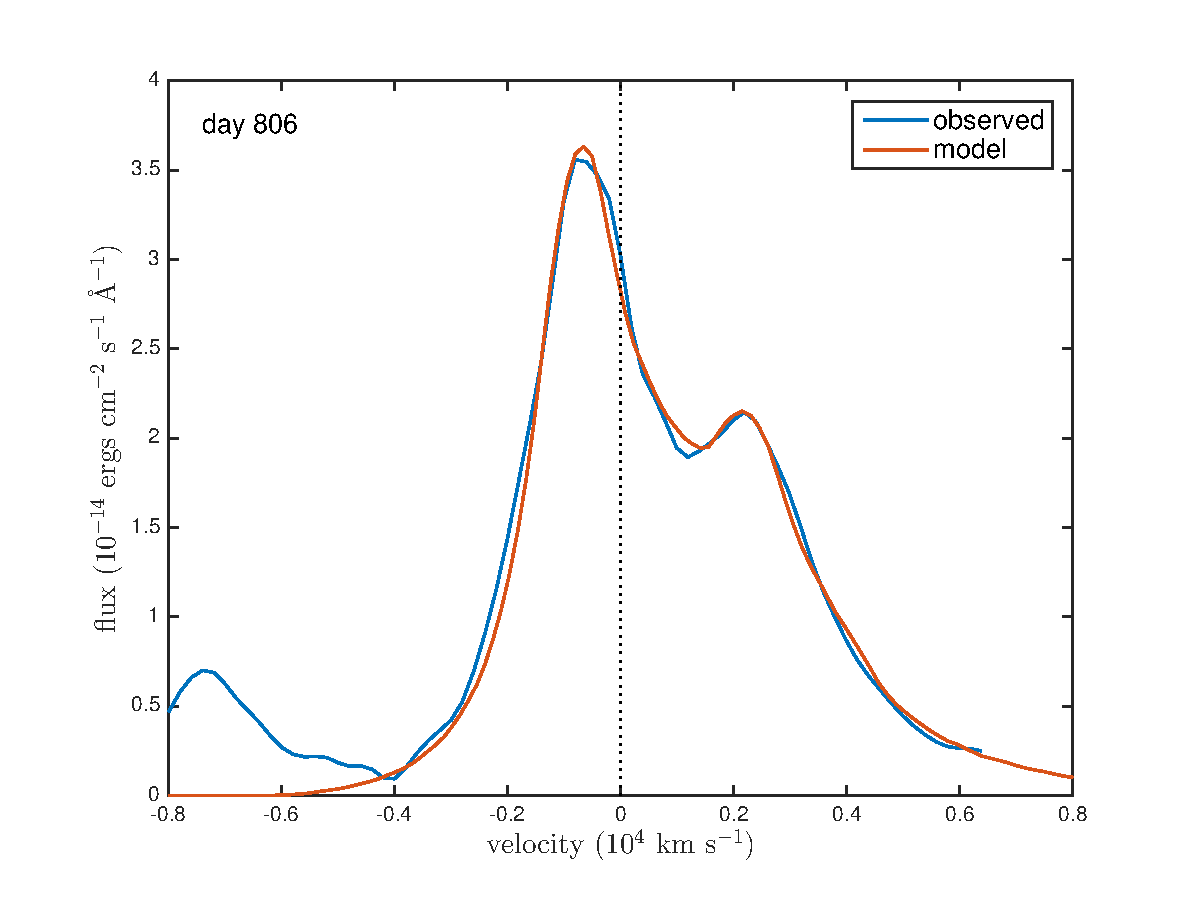
\includegraphics[trim =35 10 45 15,clip=true,scale=0.51]{clump_1/best_fit/d806OI}
\caption{Best clumped fit to the day 806 H$\alpha$ line and 
[O~{\sc i}] $\lambda$6300,6363~\AA\ doublet as per parameters detailed in Table 
\ref{clumped1}.}
\label{d806_c}
\end{center}
\end{figure*}
\subsection{Clumped Models of SN 1987A}
\label{clumped_models}
\begin{table*}
	\begin{minipage}{180mm}
	\caption{Details of the parameters used for the best fitting clumped models with $a=3.5\mu$m.}
	\label{clumped2}
	\begin{center}
  	\begin{tabular}{@{} ccccccccccl @{}}
    	\hline
  day & $v_{max}$ & $R_{in}/R_{out}$ & $\beta$ & $M_{dust}$ & $a$ & $R_{out}$ & $R_{in}$ & $\tau_{H\alpha}$ & $\tau_V$ & Figure No. \\
	& (km~s$^{-1} $) & & & ($M_{\odot}$) & ($\mu$m) & (cm) & (cm)  \\
	\hline
1862 & 8500 & 0.14 & 1.9 & 2.00E-02 & 3.50 & 1.37E+17 & 1.91E+16 & 0.85 & 1.70 & \ref{d1862_3604_cmax} \\
2875 & 9500 & 0.12 & 2 & 8.00E-02 & 3.50 & 2.36E+17 & 2.83E+16 & 1.15 & 2.30 & \ref{d1862_3604_cmax} \\
3604 & 10250 & 0.12 & 2 & 1.70E-01 & 3.50 & 3.19E+17 & 3.83E+16 & 1.33 & 2.67 & \ref{d1862_3604_cmax} \\
    \hline
  \end{tabular}
  \end{center}
\end{minipage}
\end{table*}

It has been shown through the modelling of photometric data that when dust 
is assumed to have a clumped distribution the derived masses can be 
significantly larger than if the dust is distributed smoothly between the 
inner and outer radii.  We present two sets of fits to the data based on 
the modelling used by W15.  Each fit is derived from the smooth best 
fitting model such that the packets are emitted according to a smooth 
radial density profile.  However, the dust is no longer coupled to the gas 
but instead is located entirely in clumps of size $R_{out}/30$.  The 
clumps are distributed stochastically between $R_{in}$ and $R_{out}$ with 
the probability of a given grid cell being a clump proportional to $r^{- 
\beta }$ where $i(r) \propto r^{-2 \beta}$.  The number of clumps used is 
determined by the filling factor which is kept constant at $f=0.1$.  All 
properties are fixed from the smooth models with the exception of grain 
size and dust mass.

As for fully self-consistent radiative transfer models of photometric 
data, the dust masses required to reproduce the same degree of absorption 
in a clumped setting are considerably higher than in the the smooth case.  
However, it also necessary to have a slightly larger albedo in order to 
reproduce the red side of the profiles.  This is presumably because when 
the dust is located in clumps the radiation is subject to less scattering 
as well as less absorption.  The reduction in scattering appears not to be 
compensated for by the increased dust mass and a larger grain size is 
therefore required, particularly at day 714.  A grain size of $a=0.6\mu$m 
is therefore used throughout the clumped models as the smallest possible 
grain size capable of reproducing the data reasonably. Full details of all 
parameters used for these models may be found in table \ref{clumped1} and 
the fits are presented in figures \ref{d714_c} to \ref{d1862_3604_c}.

Since these models also utilise the smallest possible grain size and 
therefore represent an approximate minimum dust mass in the case of a 
clumped distribution of amorphous carbon, we also investigate the 
potential for this method to derive an upper bound on the dust mass.  By 
steadily reducing the grain size from an initial value of 5$\mu$m 
(motivated by the maximum possible grain size derived by W15 for their day 
8515 model), we produce a set of models representing a theoretical maximal 
dust mass.  Throughout the course of our modelling it transpired that the 
grain size used for the minimum models at days 714 and 806 ($a=0.6\mu$m) 
in fact represents the best fit to the data and even a small fluctuation 
in $a$ in either direction results in a significantly poorer fit, either 
over- or underestimating the red wing and the trough in the doublet.  We 
therefore conclude that the dust mass estimates produced at days 714 and 
806 for a grain size of $a=0.6\mu$m are strong estimators of the dust mass 
at this epoch.  At later epochs however we find that equally good fits may 
be generated by substaintially larger grains with $a=3.5\mu$m (see figure 
\ref{d1862_3604_cmax}).  Details of the parameters used in these models 
presented in table \ref{clumped2}.


\subsection{Contamination of the the H$\alpha$ profiles at days 704 and 806}

The profile at day 704 exhibits several of the features discussed above.  
There is an increase in flux on the red side of the data $v>2000$~km~s$$^{-1}$ 
as a result of a dust scattering reprocessing radiation to the red.  
There is also an approximately linear section between the peak at $v=-420$ 
km~s$^{-1}$ and the very slight corner visible at $v_{min}$.  The profile 
at day 806 has similarly identifiable features with a noticeable wing on 
the red side extending out to $v=8000$ km~s$^{-1}$.  It also exhibits a 
definite shoulder reaching to $v \approx 900$ km~s$^{-1}$ which we assume 
to be the value of $v_{min}$.  In both these cases, with both smooth and 
clumped models, we struggle slightly to fit both the corner and the peak 
of the profile.  In both instances, accurately fitting the corner results 
in a peak that is slightly further towards the blue than is seen in the 
observations.  We suggest that this discrepancy, which is more noticable 
at day 806 because of the more distinctive shape of the profile, is likely 
a result of the increased flux produced by the clump at $v=-360$ 
km~s$^{-1}$.  This clump, clearly visible in the line profile at day 673 
and identified as such in the literature 
\citep{Spyromilio1993a,Hanuschik1993}, is likely contaminating the 
position of the peaks of the profiles at days 714 and 806.  The clump is 
perhaps not so clearly discernible at these epochs as a result of the poor 
resolution of the CTIO spectra but is known to persist until around day 
900 \citep{Hanuschik1993}.

\subsection{The shoulder in the H$\alpha$ line profile at day 806}

The shoulder in the H$\alpha$ line profile at day 806 has previously been 
attributed to an unresolved [NII] $\lambda$6583~\AA\ line at $v=933$ 
km~s$^{-1}$ \citep{Kozma1998}.  Narrow [N~{\sc ii}] lines at $\lambda=$ 
6583~\AA\ and $\lambda=$ 6548~\AA\ are certainly seen by day 1862 and have 
to be 
removed in order to consider the evolution of the broad H$\alpha$ profile. 
It is somewhat unfortunate that the theoretical minimum velocity falls at 
a similar velocity to this line as it makes it difficult to distinguish 
the two features.  We postulate however that this feature may in fact be a 
product of a relatively steep density profile and the formation of dust 
within the ejecta as demonstrated in both our fits (see figures 
\ref{d806bf} and \ref{d806_c}) and our investigation of the parameter 
space (see figures \ref{bt} and \ref{wt}).

It is a general challenge inherent in the nature of this modelling that 
interesting features that are present in line profiles are not necessarily 
easily identifiable.  In particular, the effects of clumping and 
asymmetrical distributions in the ejecta may cause fluctuations that are 
hard to distinguish from the potential signatures of dust formation 
discussed in section \ref{params}.  Key indicators such as symmetry in the 
location of discontinuities on the red and blue side, typical dust profile 
signatures and the presence of a red scattering wing should be considered.


\subsection{Potential challenges at later epochs: days 1862, 2875 and 3604}

At later epochs, even very tiny fluctuations in adopted value of the 
continuum level can have a substantial effect on the fit of the resulting 
profile.  Since it is not feasible to establish the level of the continuum 
so precisely, the value of the continuum has been left as a free parameter 
that may be adjusted (to within sensible margins) in order to allow for 
the widest possible dust mass range to be determined.  We generally find 
it is necessary to assume a continuum level that is slightly lower where 
the adopted dust mass is higher.

The line profiles at these later epochs are relatively noisy and have had 
substantial sections of the profile removed as a result of contamination 
by the H$\alpha$ and [NII] narrow lines.  Unfortunately, this removes a 
critical section of the line ($500$ km~s$^{-1}<v<1500$ km~s$^{-1}$) that 
would be potentially informative.  However, we do achieve excellent fits 
to the line profiles at these epochs.


\begin{figure*}
\begin{center}
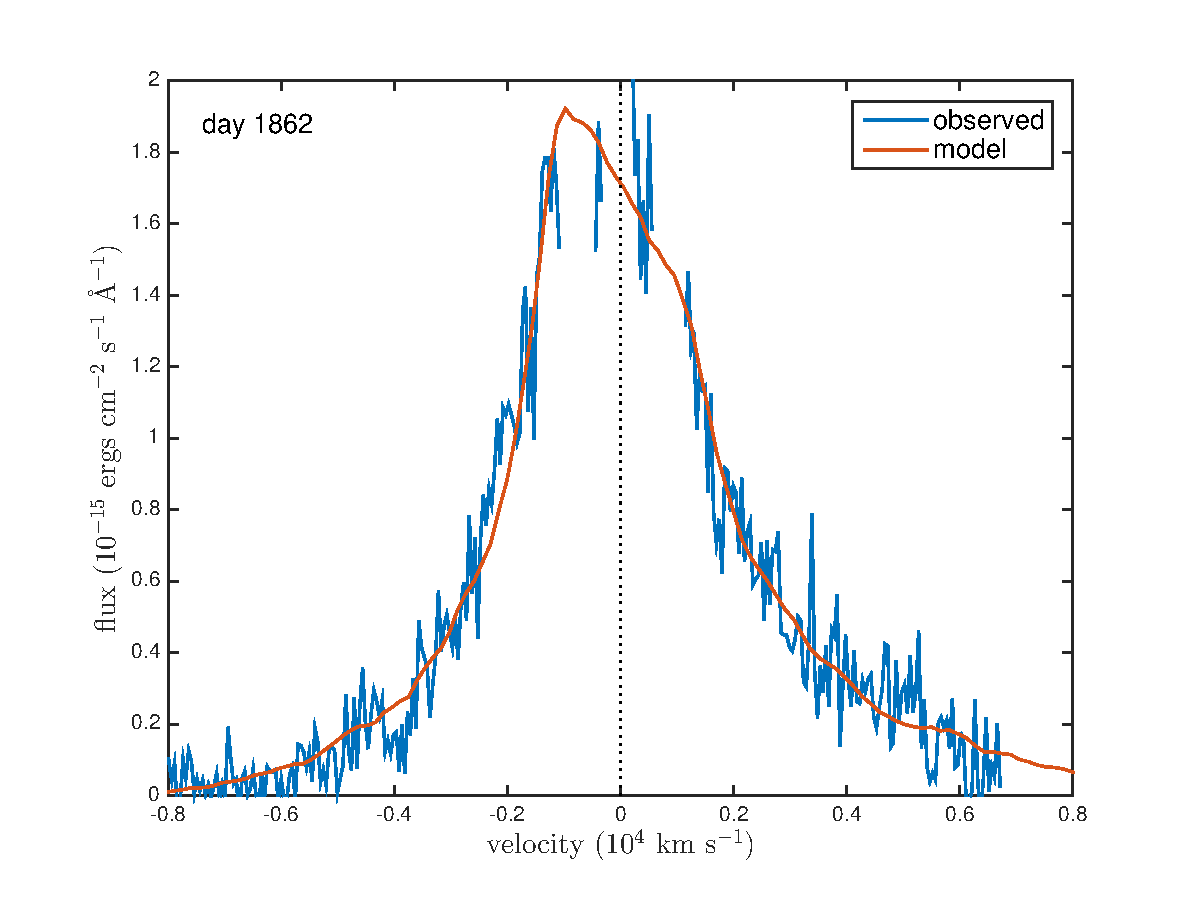
\includegraphics[trim =37 10 45 15,clip=true,scale=0.35]{clump_1/best_fit/d1862Ha}
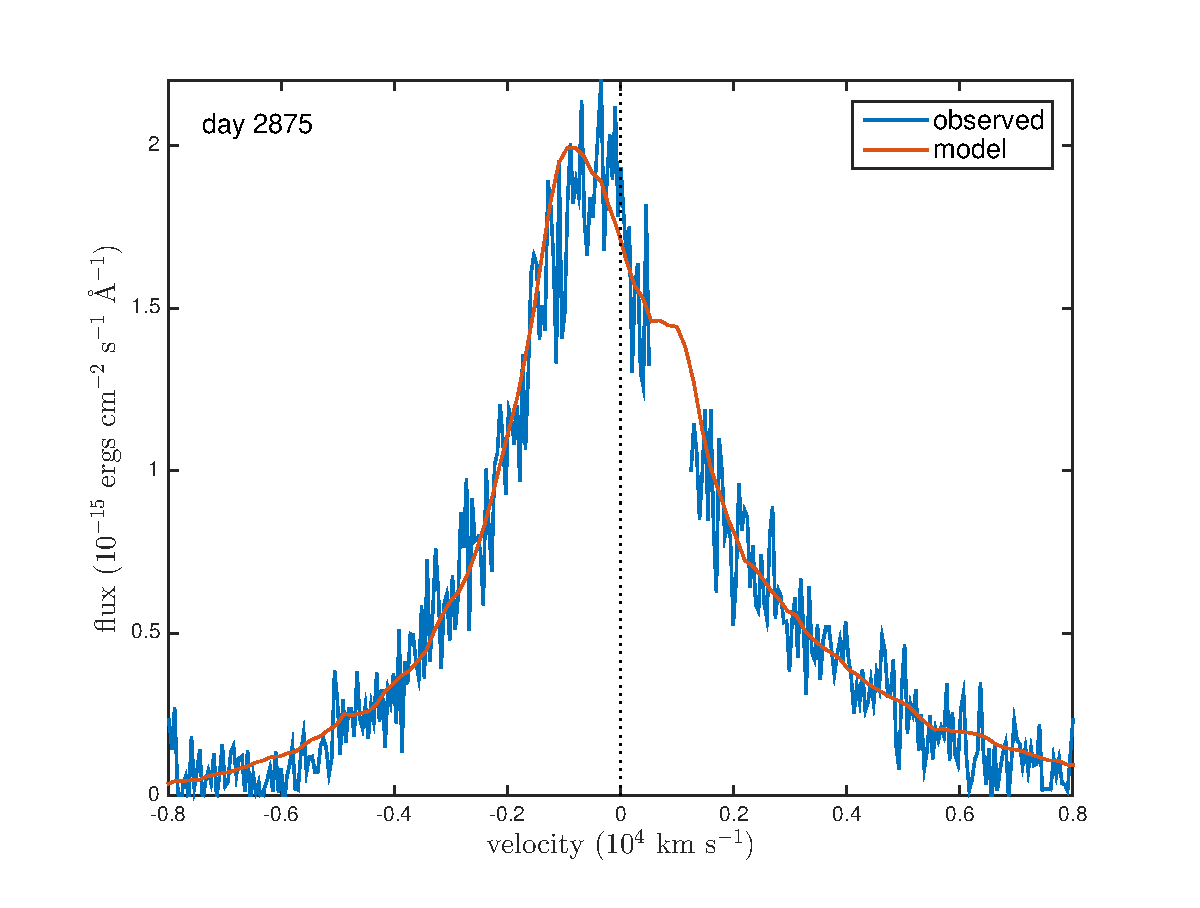
\includegraphics[trim =55 10 45 15,clip=true,scale=0.35]{clump_1/best_fit/d2875Ha}
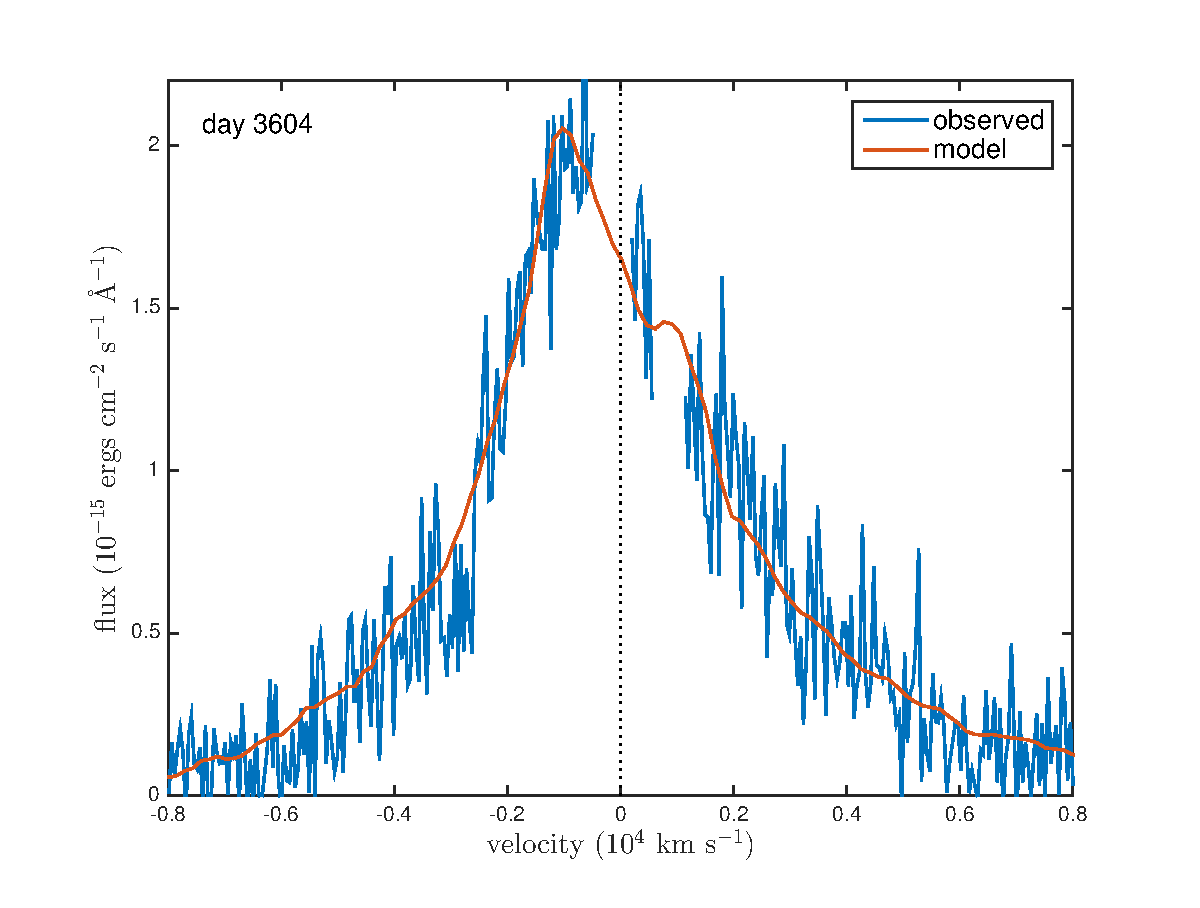
\includegraphics[trim =55 10 45 15,clip=true,scale=0.35]{clump_1/best_fit/d3604Ha}
\caption{Best clumped fit to the H$\alpha$ line at days 1862, 2875 and 
3604 as per parameters detailed in table \ref{clumped1} with $a=0.6\mu$m.}
\label{d1862_3604_c}
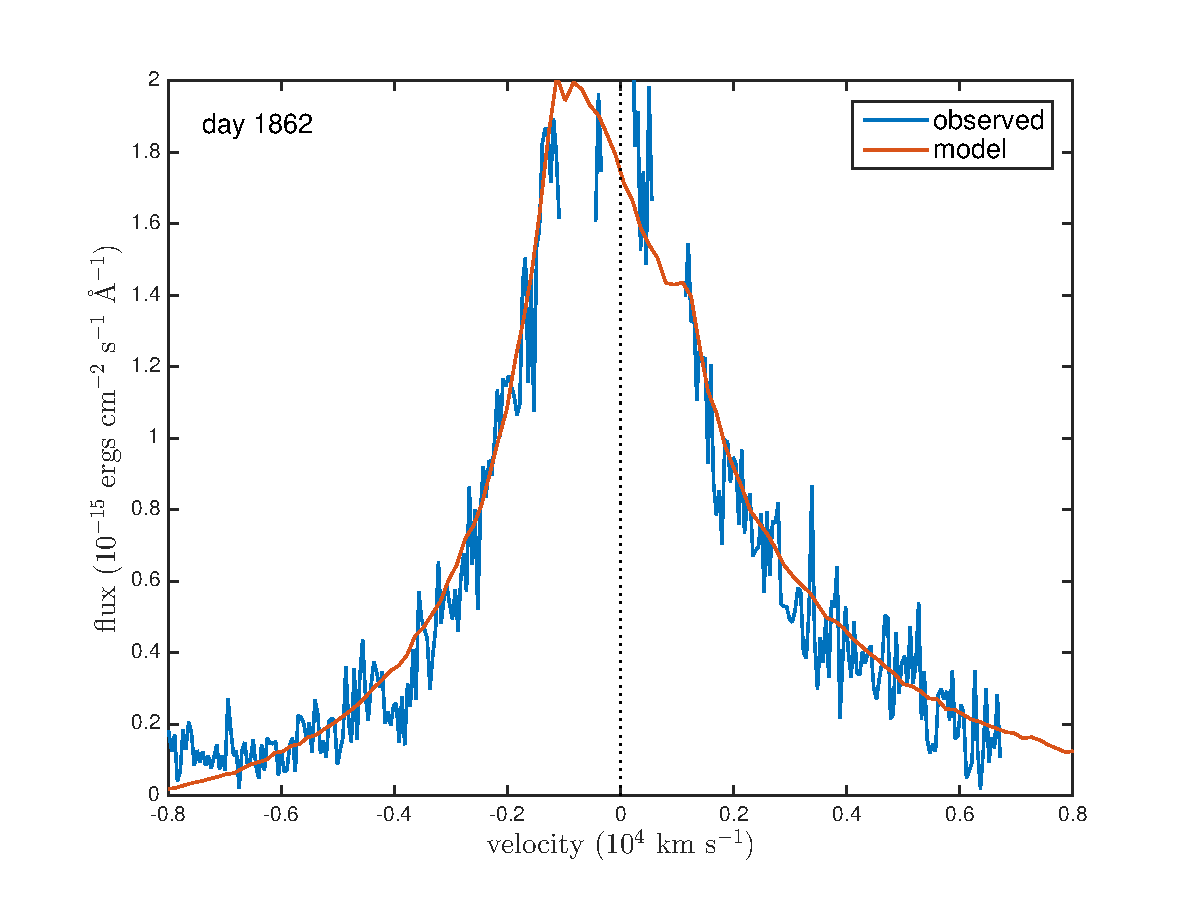
\includegraphics[trim =37 10 45 15,clip=true,scale=0.35]{clump_1/maximum/d1862Ha}
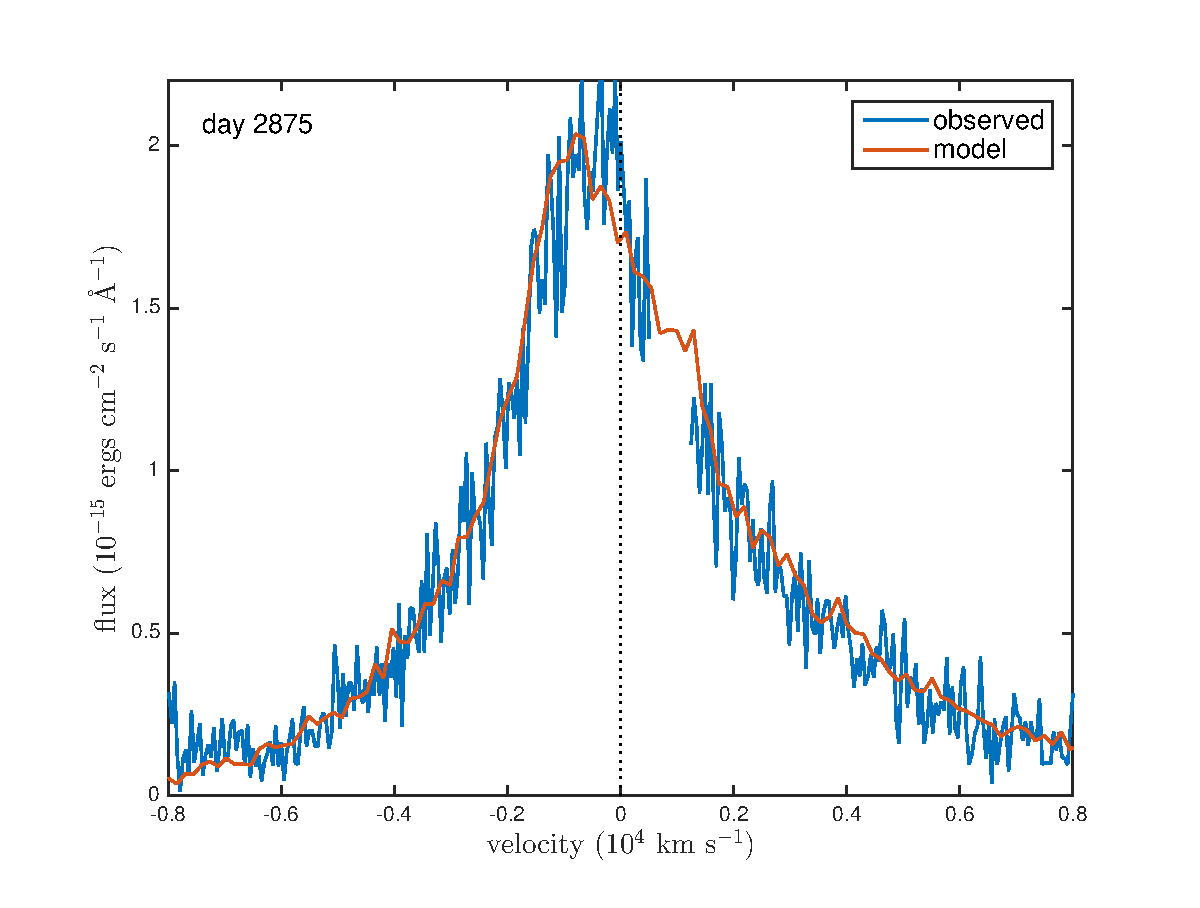
\includegraphics[trim =55 10 45 15,clip=true,scale=0.35]{clump_1/maximum/d2875Ha}
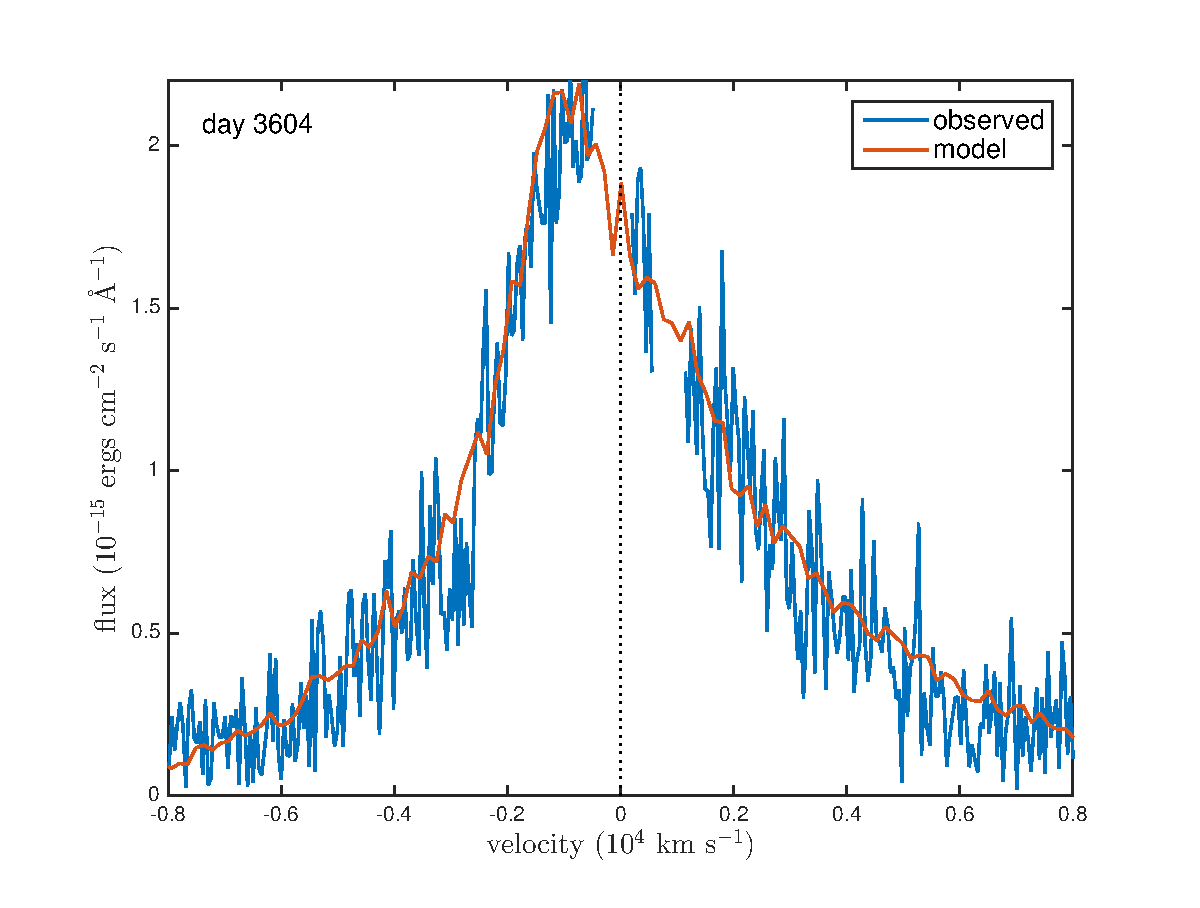
\includegraphics[trim =55 10 45 15,clip=true,scale=0.35]{clump_1/maximum/d3604Ha}
\caption{Best clumped fit to the H$\alpha$ line at days 1862, 2875 and 
3604 as per parameters detailed in table \ref{clumped2} with $a=3.5\mu$m.}
\label{d1862_3604_cmax}
\end{center}
\end{figure*}

\section{Discussion}
\label{discuss}

We have collated a range of archival spectral data in the optical and IR 
and, by modelling the evolution of the H$\alpha$ and 
[O~{\sc i}] $\lambda$6300,6363~\AA\ lines, have placed constraints on the 
evolution of newly formed dust in SN 1987A. We have done this using Monte Carlo 
models that consider both the absorbing and scattering effects of dust.  
We find dust masses that are in excellent agreement with those previously 
found at similar epochs.  We obtain large dust masses at just a few 
thousand days in agreement with the very large mass of dust deduced by 
\textit{mikako ref problem} from their observations at long wavelengths 
using Herschel. We compare our dust masses directly with those obtained by 
W15 in order to compare both their magnitude and evolution (see figure 
\ref{Mdust}).

At all epochs we find that we obtain slightly smaller dust masses than 
those of W15 although our values are still generally within the error bars 
placed on their values.  There may be a number of different reasons for 
this.  Firstly, our modelling is somewhat more conservative in its 
estimates since we use an environment of pure amorphous carbon whereas the 
models presented by W15 use a silicate fraction of 0.15 which is likely to 
increase the overall mass of dust required to produce the same 
observations, both in the case of radiative transfer SED modelling and 
line profile modelling.  Secondly, we use different sets of optical 
constants; we have used the optical constants derive by \cite{Zubko1996} 
from their BE sample where W15 use constants from 
\cite{Hanner1988}\textit{hanner ref problem}.  They state that in order to 
fit their data at early epochs (day 615) with the Zubko ACH2 sample 
smaller inner and outer radii are needed and half as much dust ($5.0 
\times 10^{-4}M_{\odot}$) is required.  This is considerably closer to the 
values we derive at similar epochs.

The other significant difference between our models is the adopted grain 
size distribution.  W15 generate fits to their ealy data using an MRN 
distribution between 0.005$\mu$m and 0.25$\mu$m in size.  They cannot 
obtain a fit with grains of $\sim 1.0 \mu$m in size at early epochs.  
However, they do not consider values in between these size point as we 
conclude is likely the case with grain sizes of $a \approx 0.6\mu$m.  For 
SED modelling it is generally the case that the larger the grain size 
used, the less dust is required to produce the same level of flux and it 
may therefore be this difference that is generating the discrepancy in our 
results.  W15 use this property to derive a maximum possible grain size at 
late epochs as well and conclude that grains cannot be larger than $\sim 
5\mu$m by day 8515.  This is directly in line with the maximum grain sizes 
we derive at slightly earlier epochs.  We find that the grain size likely 
cannot have exceeded $\sim 3.5\mu$m at day 3604 and the dust masses that 
we generate using this value are very similar to the value of the W15 
sigmoid fit at this epoch.


\begin{figure*}
\begin{center}
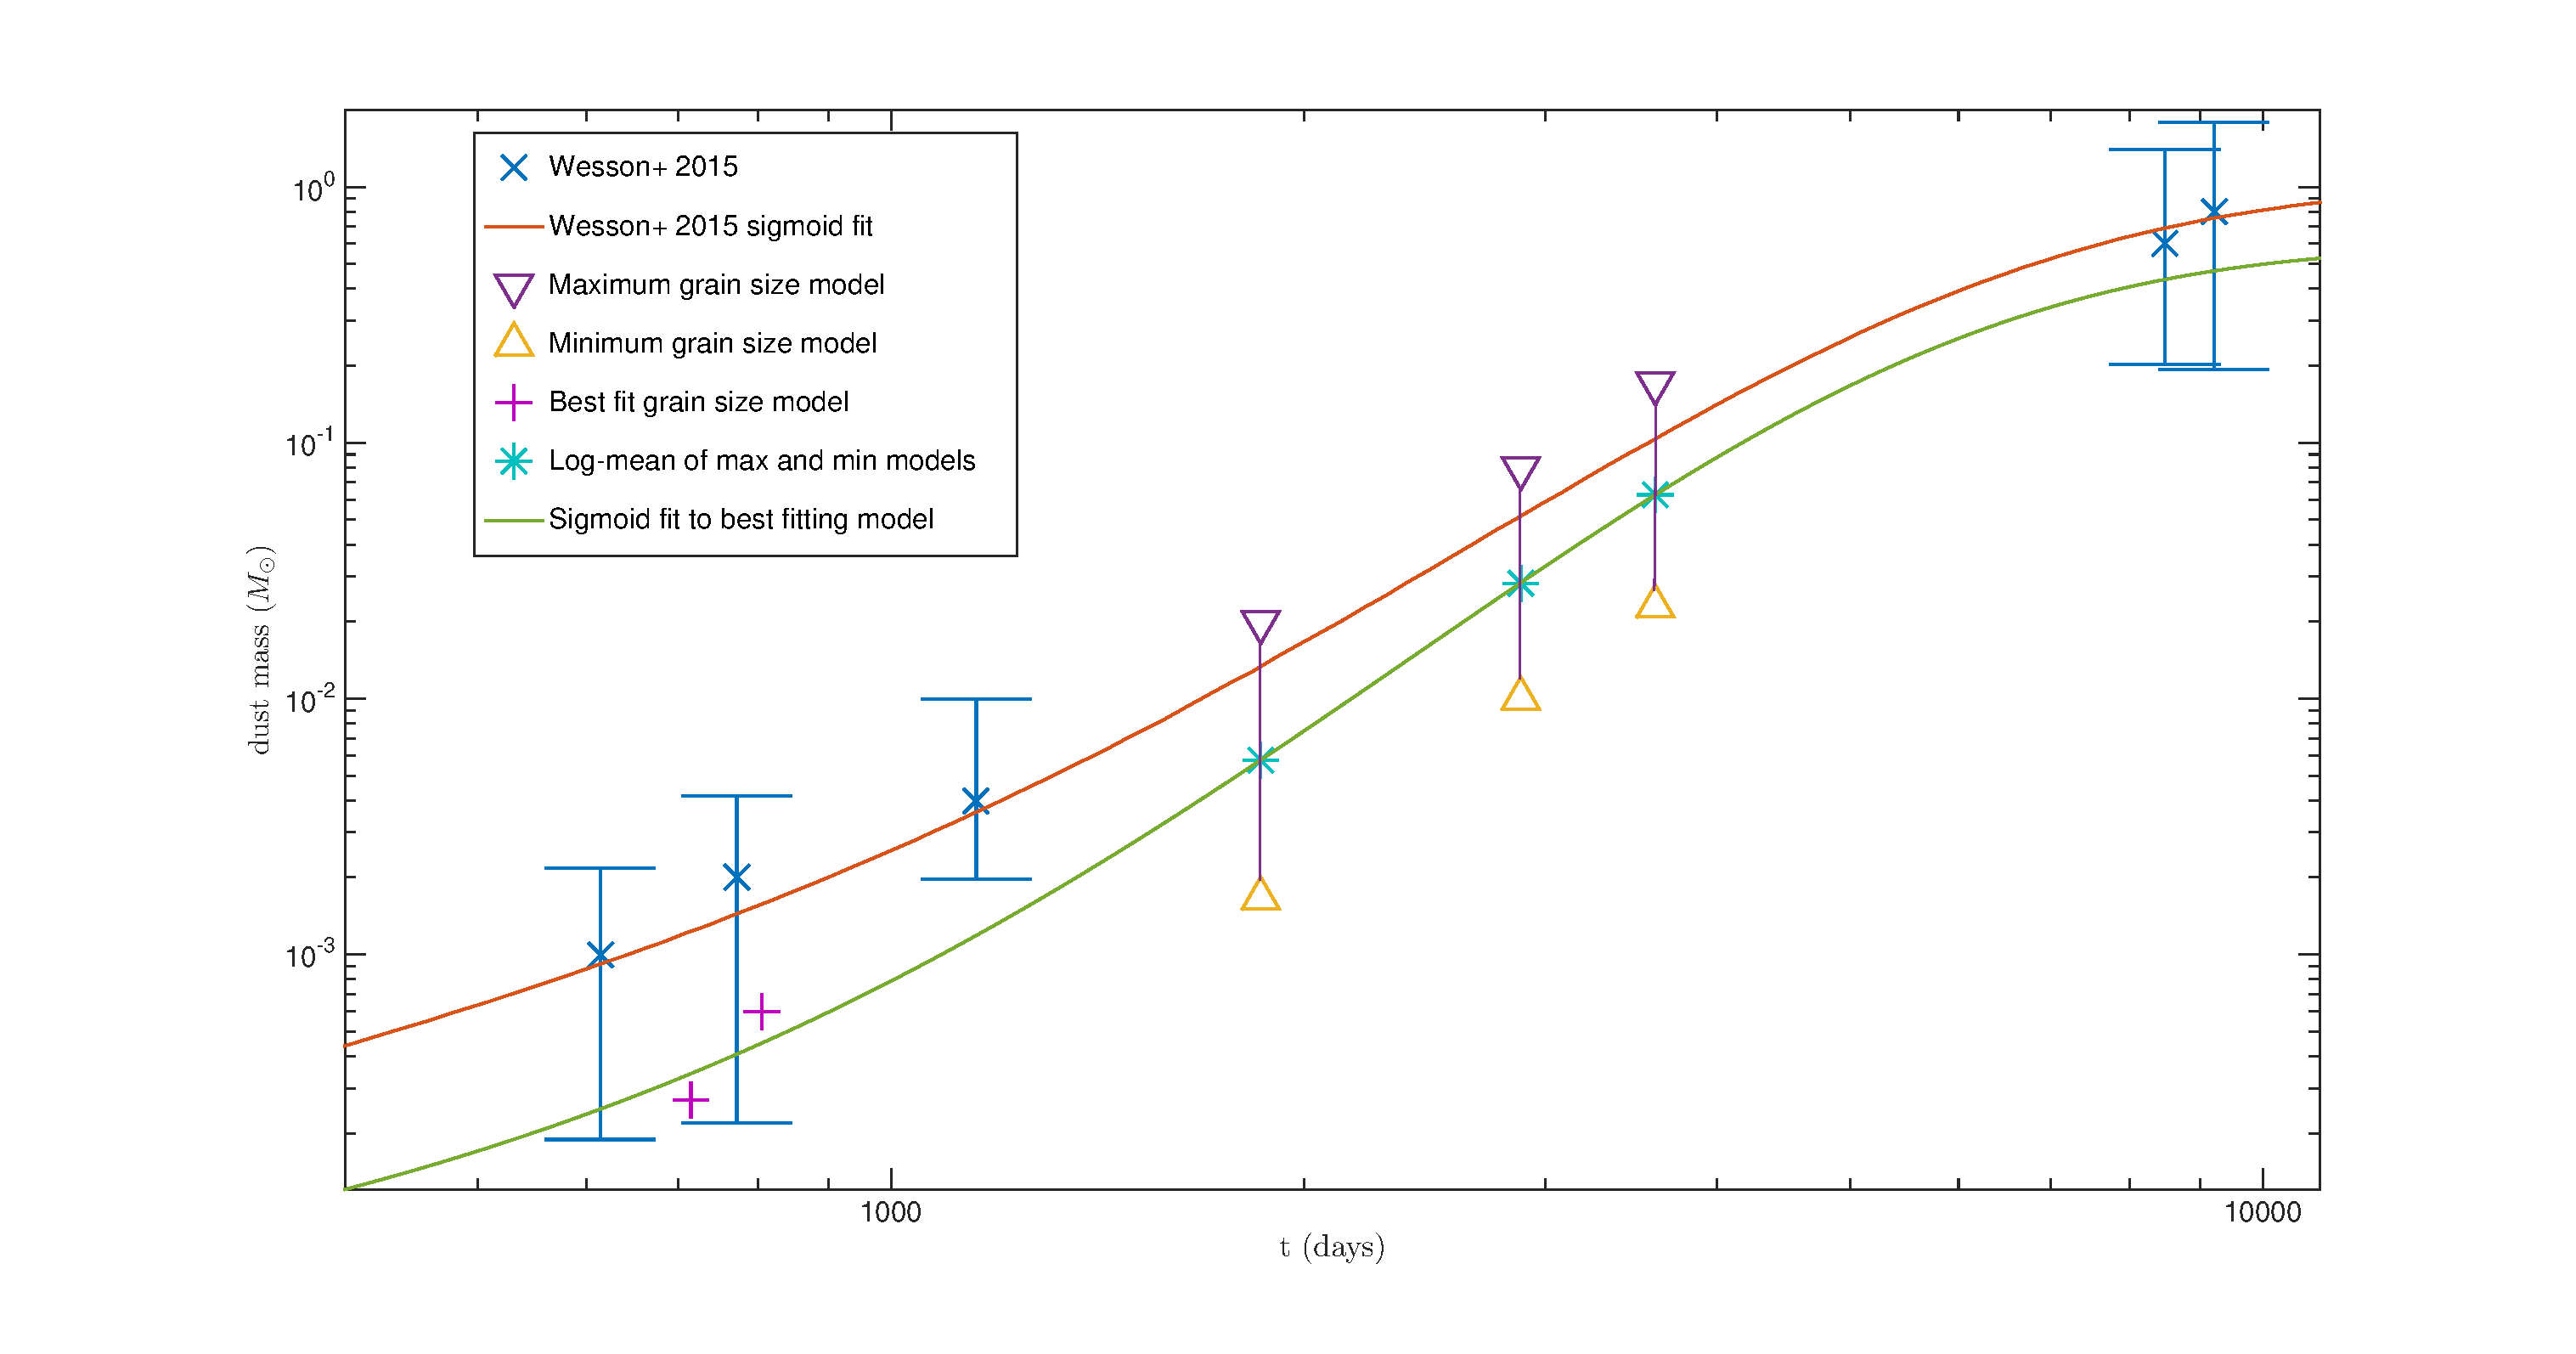
\includegraphics[trim =37 10 45 15,clip=true,scale=0.4]{Mdust_evol2}
\caption{\textit{Purple and yellow triangles -} Maximum ($a=3.5\mu$m) and 
minimum ($a=0.6\mu$m) dust masses respectively.  Values are from the 
later epoch ($t>1862$ days) clumped models of H$\alpha$.  \textit{Pink 
crosses - } Predicted dust masses (clumped models of the 
[O~{\sc i}] $\lambda$6300,6363~\AA\ doublet with grain size $a=0.6\mu$m).  
\textit{Turquoise stars -} Predicted dust masses calculated as a log 
average of the maximum and minimum values.  \textit{Green -} Sigmoid fit 
to our predicted dust masses. \textit{Blue - } dust masses derived by W15 
in their photometric modelling of SN 1987A. \textit{Red} - sigmoid fit to 
the W15 values.}
\label{Mdust}
\end{center}
\end{figure*}

Determining the relationship between the size of dust grains in the ejecta 
and the time post-explosion is important for understanding the likelihood 
of dust surviving the passage of the reverse shock travelling back through 
the ejecta. By the time the reverse shock begins to appear in the line 
profiles (around day 5000), our models predict that the grains could 
already be as large as several microns in radius but are certainly larger 
than $\sim 0.6\mu$m.  Grains larger than $\sim 0.2\mu$m are likely to 
survive and thus the majority of the dust produced is likely to survive 
(remembering that our modelling only considers an average grain size and 
makes no comment about the grain size distribution).  It has recently been 
suggested that very large grains (up to 4.2$\mu$m) may have formed in the 
ejecta of SN 2010jl very soon after the explosion (a few hundred days) 
\cite{Gall2014}.  Whilst the values we suggest are not as high that 
postulated by \citet{Gall2014}, they maintain a distribution that remains 
steeped towards the smaller end of the scale and thus, as our models only 
treat a single, average grain size, these values may be not be at odds.  
Certainly, both results suggest that grains large enough to survive the 
destructive force of the reverse shock have formed by a few hundred days 
post-explosion.

There is now a firm consensus that a very large quantity of dust has 
formed in SN 1987A between the time of the original explosion and the 
present day.  Perhaps more important therefore is the manner of its 
evolution.  We have shown that dust masses have reached the order of 
$0.1M_{\odot}$ by day 3604.  However, it is known that values several 
times as large as this are ultimately expected and thus a substantial 
fraction of the dust is likely to form after this epoch.  This is in 
strong agreement with the results produced by W15.  They derive a sigmoid 
fit to their dust mass evolution of the form

\[
M_d(t)=ae^{be^{ct}}
\]
 
where they obtain values of $a=1.0M_{\odot}$ (representing the maximum 
dust mass), $b=-8.53$ and $c=-0.000366$.  Both their dust masses and this 
sigmoid fit are shown in figure \ref{Mdust}.  This exhibits an initial 
period of slow growth followed by an intermediary period of acceleration 
followed by another slowing until a plateau is ultimately reached.  In 
this sense it may be relatively representative of the process of dust 
formation whereby initial conditions appropriate for grain growth 
gradually develop until optimal conditions are reached at an intermediate 
epoch when grain growth is at its fastest before conditions once again 
deteriorate and the rate slows again (as discussed by W15).  Performing a 
least-squares regression to this function using our predicted dust masses, 
we derive a sigmoid fit with coefficients $a=0.58M_{\odot}$, $b=-10.02$ 
and $c=-0.000416$.  These values are remarkably similar to those derived 
by W15 although the final predicted dust mass is slightly smaller in our 
case.  This sigmoid fit is also plotted in figure \ref{Mdust}.

Our modelling concurs with the suggestion of W15 that even after 
$\sim$3000 days the dust mass is only a very small fraction of its final 
value.  This is in contrast to \citet{Sarangi2015} whose chemistry models 
predict that the evolution of dust formation will have reached its plateau 
by around 5 years after the explosion first occured.

Ideally, our models would cover the entire evolution of SN 1987A right up 
to the present day.  However, the excitation of gas in the outer edges of 
the ejecta by the reverse shock after $\sim$ day 500 results in a 
significant, broad and asymmetric flux that dominates the original line 
profile.  In addition to this, the narrow lines from the ring start to 
become so significant relative to the original broad H$\alpha$ profile 
that, post-removal, there is not enough of the broad profile remaining to 
be able reliably infer information from its features.  These are factors 
that are likely to be common to most core collapse supernovae and thus are 
likely to have an impact on the wider applicability of this particular 
technique at later epochs.  Care should also be taken in the future to 
ensure that the line profiles are the temporally appropriate profile and 
not in fact a product of a light echo representing the state of the ejecta 
at some previous epoch.  Nonetheless, this technique has proved effective 
in determining dust masses formed in core-collapse supernovae through the 
detailed modelling of asymmetric line profiles and clearly has wider 
application to multiple supernovae and supernova remnants.


\section{Conclusions}

We have discussed in section \ref{params} the various potential effects of 
dust scattering and absorption on the generic shape of a line profile and 
the different features that may be produced.  In particular, attention 
should be paid to the fact that the classical blue-shifted peak and 
asymmetric profile with most flux on the blue side is very much not the 
only profile that signifies the presence of dust.  Profiles may also have 
the majority of their flux on the red side in the case of strong 
scatterers.  They will often exhibit an extended red scattering wing 
although care should be taken to first ascertain that this cannot be 
accounted for by electron scattering. It is feasible that a pronounced 
shoulder or corner may be present on the red side of the profile located 
at the minimum velocity of the shell.  This feature may often be mistaken 
for a narrow line, a product of a lack of resolution or a geometrical 
effect.

We have modelled H$\alpha$ and [O~{\sc i}] $\lambda$6300,6363~\AA\ line 
profiles 
from SN 1987A over a range of epochs and obtained dust masses of the order 
of $0.1M_{\odot}$ by day 3604.  We derive a sigmoid fit to this data that 
predicts a final dust mass of 0.68$M_{\odot}$ in line with both other 
predictions and current dust mass estimates for SN 1987A.  We conclude 
that large grains are necessary in order to reproduce the extended red 
scattering wing and asymmetry seen in several of the lines and that grains 
larger than $0.6\mu$m have formed by day 604.

We have demonstrated the efficacy of the DAMOCLES code for determining 
dust masses and established its potential for application to other 
supernovae and spectra, both archival and current.


\section*{Acknowledgments}

AB would like to thank Dr Jeremy Yates for discussions and advice during 
the development of the DAMOCLES code.  We thank Dr Raylee Stathakis for 
providing us with the AAT spectra of SN~1987A. AB's work has been 
supported by a Science and Technology Facilities Council Research 
Studentship.

\texit{ArchiveRerences}

\bibliography{87A_paper}{}
\bibliographystyle{mn2e}

\appendix

\section[]{Appendix A}

Since the outflow velocities in supernovae are high, the photon packets 
are subject to Doppler shifting at emission and at each scattering event.  
When the packet is initially emitted, it has a frequency and a trajectory 
in the rest frame of the emitter. Both of these must be transformed to the 
observer's frame in order for the packet to be propagated through the 
grid.  The new direction and frequency in the observer's frame may be 
simply found by transforming the momentum 4-vector $\mathbf{P}$ which is 
defined as

\begin{equation}
\mathbf{P}=
\begin{pmatrix}
	E \\
	p_x \\
	p_y \\
	p_z \\
	\end{pmatrix} =
	\begin{pmatrix}
	h \nu \\
	h \nu x \\
	h \nu y \\
	h \nu z \\
	\end{pmatrix}
\end{equation}


\noindent We may then derive $\mathbf{P'}$, the momentum 4-vector in the 
observer's frame using the relation

\begin{equation}
	\mathbf{P'}=\Lambda \mathbf{P}	
\end{equation}

\noindent where 

\[
	{\Lambda}=
	 \begin{pmatrix} 
	  \gamma & -\gamma \beta_x & -\gamma \beta_y & -\gamma \beta_z \\
	 -\gamma \beta_x & 1+(\gamma-1)\frac{\beta_x^2}{\beta^2} & (\gamma-1)\frac{\beta_x \beta_y}{\beta^2} & (\gamma-1)\frac{\beta_x \beta_z}{\beta^2} \\
	 -\gamma \beta_y  & (\gamma-1)\frac{\beta_y \beta_x}{\beta^2} & 1+(\gamma-1)\frac{\beta_y^2}{\beta^2} & (\gamma-1)\frac{\beta_y \beta_z}{\beta^2} \\
	 -\gamma \beta_z & (\gamma-1)\frac{\beta_z \beta_x}{\beta^2} & (\gamma-1)\frac{\beta_z \beta_y}{\beta^2} & 1+(\gamma-1)\frac{\beta_z^2}{\beta^2} \\
	 \end{pmatrix}
\]

 \noindent and $\mathbf{\beta}=\frac{{\bf{v}}}{c}$,   $\mathbf{\beta}=(\beta_x,\beta_y,\beta_z)$,   $\beta=\mathbf{\beta}$ and $\gamma = \frac{1}{\sqrt{1-\beta^2}}$.


In practice, the velocities considered are low enough that it is 
unnecessary to consider terms of order $O(\frac{v^2}{c^2})$ and thus 
${\Lambda}$ may be reduced to

\begin{equation}
	{\Lambda}=
	 \begin{pmatrix} 
	 1 \& - \beta_x & - \beta_y & - \beta_z \\
	- \beta_x & 1 & 0 & 0 \\
	- \beta_y  & 0 & 1 & 0\\
	- \beta_z & 0 & 0 & 1 \\
	 \end{pmatrix}
	 \\
\end{equation}

\noindent The new direction of travel and frequency in the observer's 
frame are therefore given by  
\begin{equation}
\nu'=\nu(1-x\beta_x-y\beta_y-z\beta_z) \\
\end{equation}
\[
x'=\frac{\nu}{\nu'}(x-\beta_x) 
\]
\[
y'=\frac{\nu}{\nu'}(x-\beta_y) 
\]
\[
z'=\frac{\nu}{\nu'}(x-\beta_z) 
\]

For each scattering event, the packet must be transformed both into and 
out of the comoving frame. The reverse transform is applied by using the 
inverse Lorentz matrix $\Lambda^{-1}$ which is obtained by reversing the 
sign of $\bf{v}$.  Positive $\bf{v}$ is defined for frames moving away 
from each other and thus $\bf{v}$ is defined to be negative in the 
direction of the observer.

\bsp

\label{lastpage}

\end{document}
